\documentclass[a4paper,10pt,notitlepage]{report}

\usepackage[utf8]{inputenc}
\usepackage{fullpage}
\DeclareFontShape{OT1}{cmtt}{bx}{n}{<5><6><7><8><9><10><10.95><12><14.4><17.28><20.74><24.88>cmttb10}{}
\usepackage{listings}
\usepackage{graphicx}
\usepackage{float}
\usepackage{parcolumns}
\usepackage{qtree}
\usepackage{url}
\usepackage[protrusion=true,expansion=true]{microtype}

\usepackage{color}
\usepackage{xcolor}
\usepackage{caption}
\usepackage{textcomp}
\usepackage{todonotes}
\usepackage{tikz}
\usepackage{tikz}
\usetikzlibrary{calc}
\newcommand{\tikzmark}[1]{\tikz[overlay,remember picture] \node (#1) {};}

\title{Detouring program execution in binary applications \\
{\large MEng Final Report}}
\author{Mike Kwan \texttt{mk08}\\
Department of Computing,\\
Imperial College London\\
\texttt{michael.kwan08@imperial.ac.uk}}

\lstset{
  language=C,
  captionpos=b,
  basicstyle=\small\ttfamily,
  commentstyle=\textit,
  keywordstyle=\bfseries,
%  numbers=left,
  numberstyle=\tiny,
  numbersep=5pt,
%  escapeinside={/*@}{@*/},b
  tabsize=2,
  breaklines=true,
  extendedchars=true,
  columns=fullflexible,
  xleftmargin=16pt,
  showspaces=false,
  showtabs=false,
  showstringspaces=false,
  mathescape
}

\begin{document}
\maketitle
\tableofcontents

\chapter{Introduction}\label{chap:Introduction}

The ability to modify the behaviour of an executable is a powerful aspect of software development that is often not fully exploited. While editing the source code of executables is a routine practice in software development, there are many cases where there is either no access to source code or it is inconvenient to perform modifications at that level.

One such example is the situation where a bug is displayed only in the production environment. The classical approach is to recompile the code with integrated logging and to reproduce the bug. This allows a developer to isolate and gather information about the circumstances under which the bug occurs and to `catch it in the act'. Unfortunately, this is often impractical if the system under test is already in production. Furthermore, when deployment is a heavyweight process, giving a user a logged or debug build can be cumbersome and disruptive.

An ideal solution would be to have some form of injectable logging which can be performed by an end-user in a manner that resembles the weaving of aspects in aspect-oriented programming. That is, the cross-cutting behaviour of logging becomes modularised. In our exemplary scenario, the user would run some tool which patches logging functionality to the target system, either altering it or duplicating it and altering the copy. The following example illustrates what such a tool would allow us to achieve. Given the target system:

\begin{lstlisting}[language=C,caption={Target Process}]
#include <stdlib.h>
#include <time.h>

int func1(int num)
{
  return 10/num;
}

int main(void)
{
  srand(time(NULL));

  for(int i=0; i<5; i++) {
    func1(rand() % 5);
  }

  return EXIT_SUCCESS;
}
\end{lstlisting}

In this circumstance, \emph{rand() \% 5} will occassionally evaluate to 0 leading to \emph{func1} performing a divide-by-zero causing the FPU to signal a hardware exception. The tool should allow a user to determine whether \texttt{func1} was invoked, and if so when, how many times and with what parameters/return values.

As a concrete real-world example, the issue tracker of \emph{lighttpd} illustrates several cases with the exact scenario we are describing\footnote{Bug \#1278 (http://redmine.lighttpd.net/issues/1278)}\footnote{Bug \#1116 (http://redmine.lighttpd.net/issues/1116)}\footnote{Bug \#605 (http://redmine.lighttpd.net/issues/605)}. The tool would make it possible to provide users with a piece of code which would be injected into the binary. The tool would then patch the binary to make calls to the injected code which would collect the information necessary to hunt down the bug. Observation through tracing is only a single use of a tool capable of injecting arbitrary code into a binary. Execution detouring is not a new concept and previous example usages include:

\begin{enumerate}
 \item \textbf{Debugging} - \emph{IF} is a Windows tool instrumenting \emph{Microsoft Detours} into a stealthy debugger. The tool provides the emulation of breakpoints through execution detouring rather than using standard implementations of software and hardware breakpoints\cite{IF}. IF provides users with the ability to target an executable and mine information on the data/code flow, order of execution and parameters/return values of functions. 
 \item \textbf{Profiling} - Detouring has been used extensively for profiling and tracing. Notable implementations include \emph{Valgrind}, \emph{pixie} and \emph{qpt}\cite{qpt,qpt_pixie,valgrind}, which inject instrumentation to record execution frequencies and trace memory references.
 \item \textbf{Interception} - \emph{NOZZLE} is a tool which performs runtime heap-spraying detection\cite{nozzle} through the use of detouring. Once again, it is implemented on top of \emph{Microsoft Detours}. The tool intercepts calls to the memory manager in the Mozilla Firefox browser.
\end{enumerate}

We want to be able to perform execution detouring on Linux x86-32 and x86-64, where related work is relatively sparse. Essentially, Microsoft Detours exists as the de facto standard for execution detouring on the Windows platform, whereas there is no such tool for Linux. Some existing solutions on Linux appeared to be potentially promising but were later dismissed for reasons such as discontinued development or having unnecessarily complex interfaces which were difficult to use. The latter is certainly true of several solutions which provide limited support for detouring but are unpopular, mainly because they are large toolchains simply incorporating detouring as one of many provided features. For this reason, their usage is cumbersome and their API complicated (compared to Microsoft Detours).

\section{Requirements}
\label{sec:Requirements}

We intend to produce a lightweight and dedicated library for Linux x86-32 and x86-64 which provides execution detouring functionality for existing binaries where source code is unavailable. The intended library will \emph{(F1)} allow users to override arbitrary functions with user defined routines. Furthermore, the library must  \emph{(F2)} provide the capability to extend the semantics of functions in the original code through trampolining (see \emph{section \ref{sec:trampoline}}). These features work at the procedural level, but the library should also \emph{(F3)} expose an interface that allows modification (insertion, modification and removal of instructions) at the basic-block level. The library will provide access to these features through a simple and clean interface which abstracts implementation details.

In order to be convenient to a user, the library will perform analysis on the target binary to enumerate routines and the basic blocks within them. This analysis should take advantage of any available symbol information. To effectively represent the target, \emph{(F4)} a control flow graph should be generated in the form of a directed graph. A visitor pattern is ideal for traversing such a graph:

\begin{lstlisting}[language=C,caption={API for traversal of control flow graph},label={lst:VisitorPattern}]
bf_enum_basic_blk(struct bin_file * bf, void (*handler)(struct bin_file *, struct bf_basic_blk *, void *), void * param);
\end{lstlisting}

\emph{Listing \ref{lst:VisitorPattern}} illustrates an example of the proposed API for modifying basic blocks. The \texttt{handler} passed into the function will be called as each basic block in the binary is traversed. As is common with the usage of C callbacks, the user is able to provide a parameter which will be passed to the handler function for each invocation. Multiple values can be passed by aggregating them into a \emph{struct} and passing a pointer to it. The API will provide similar variants for handling the enumeration and traversal of procedures and instructions. We will provide another set of functions which give \emph{(F5)} direct access to the generated control flow graph. This will allow people to build further on top of the library, such as creating a tool to analyse the differences between two binaries by examining and comparing their respective control flow graphs.

One specific use of the library is within an existing project, which has its own runtime environment. This means an optimal solution would \emph{(F6)} require no extra runtime requirements or separate environment to be distributed.

We plan to \emph{(F7)} re-use as much existing functionality as possible to simplify the development and future maintenance. This means making optimal use of relevant libraries that we find.

\section{Report Structure}

We start by taking a deeper look into some of the technical specificities of related concepts in Background (Chapter~\ref{chap:Background}). This will help with understanding what considerations we must bear in mind. This will also enable us to examine related work more critically and ultimately justify planning and design decisions we make. After this, Related Work (Chapter~\ref{chap:Related}) will discuss in further detail the existing work that has been done in this field. We will present our findings and discuss why we assessed existing solutions to be unsuitable. As well as this, we will look at what we can take away from these solutions.

In Design (Chapter~\ref{chap:Design}), we will review the functional requirements defined in Requirements (Section~\ref{sec:Requirements}) and discuss our intended approach and the proposed solution. The architecture of the solution is discussed and a high-level view of its constituent components presented in Architecture (Chapter~\ref{chap:Architecture}). The actual implementation is discussed in Implementation (Chapter~\ref{chap:Implementation}), where the details about how the library works from a technical aspect are revealed. This section will also cover the optimisations that were made to the library. Any major deviations between the original design and the actual implementation are highlighted here.

Workflow (Chapter~\ref{chap:Workflow}) gives the general usage and workflow with the library. The aim is to show the expressibility and ease-of-use of the library interface compared to existing software.

The final solution must work robustly and not just for toy examples. The library contains a test suite which is discussed in Testing (Chapter~\ref{chap:Testing}). The Evaluation (Chapter~\ref{chap:Evaluation}) benchmarks the success of the project. We also discuss the limitations of the library. Finally, the Conclusion (Chapter~\ref{chap:Conclusion}) concludes the project and discusses future work.
\section{Background}

Execution detouring is widely used throughout the industry with established library implementations already existing. As well as considering related work and why they do not meet our requirements, this section will discuss common methods of detouring. We will also provide the intuition for many of the design decisions of the project by covering the relevant technical details of an executable's life cycle.

\subsection{Detouring}

From a simplified technical viewpoint, a detour is set by replacing the first few instructions of a target function with an unconditional jump to a user-provided detour function. In this way the code path can be redirected for all given calls to some function.

\begin{parcolumns}[nofirstindent]{2}
 \colchunk{
  \noindent\begin{minipage}{.45\textwidth}

\begin{lstlisting}[language={[x86masm]Assembler},caption={Original code},label={lst:OrigCode},columns=fixed]
TargetFunction:
  PUSH EBP $\tikzmark{L1line1}$
  MOV EBP, ESP
  SUB ESP, 0x0C0
  PUSH EBX $\tikzmark{L1line2}$
  PUSH ESI
  ...
  RET
\end{lstlisting}

  \end{minipage}
 }
 \colchunk{
  \begin{minipage}{.45\textwidth}

\begin{lstlisting}[language={[x86masm]Assembler},caption={Code after insertion of detour},label={lst:AfterDetour},columns=fixed]
TargetFunction:
$\tikzmark{L2line1}$  JMP Instrumentation
  NOP
  NOP
  NOP
  NOP
$\tikzmark{L2line2}$  PUSH EBX
  PUSH ESI
  ...
  RET

Instrumentation:
  ...
  RET
\end{lstlisting}

  \end{minipage}
 }
 \colplacechunks
\end{parcolumns}

\tikz[overlay,remember picture,-latex] \draw[dashed,thick,out=0,in=160,color=black,->] ($(L1line1)+(0pt,0.7ex)$) to ($(L2line1)+(0pt,0.7ex)$);
\tikz[overlay,remember picture,-latex] \draw[dashed,thick,out=0,in=200,color=black,->] ($(L1line2)+(0pt,0.7ex)$) to ($(L2line2)+(0pt,0.7ex)$);

\emph{Listing \ref{lst:OrigCode}} and \emph{\ref{lst:AfterDetour}} illustrate a detouring example in x86-32. The x86-64 implementation is conceptually identical but has minor technicalities that must be considered. Both architectures use variable length instructions, which poses a problem for code patching. On x86-32, the \textbf{JMP} instruction is five bytes long and in this example, patching it in places a new instruction boundary between the \textbf{SUB ESP, 0x0C0} and \textbf{PUSH EBX} instructions. The \textbf{SUB ESP, 0x0C0} instruction is partially overwritten, and its preceding instructions completely overwritten. For clarity, we have padded the bytes after the \textbf{JMP} up to the immediately subsequent instruction with \textbf{NOP} even though this is not functionally necessary. The padding has replaced the end of the partially overwritten instruction which would otherwise contain garbage bytes.

When a function is called, the address of the instruction after the \textbf{CALL} is pushed on the stack as the return address. Since the new code does not modify the stack, \emph{Instrumentation} will return using the original return address from the call to \emph{TargetFunction}.

Other methods of detouring exist but are less widely used. For example, instead of patching the target function, all calls to it can be replaced instead. However, to be reliable this technique requires substantial symbolic information which is not commonly available at the binary level.

\subsubsection{Trampoline} \label{sec:trampoline}
Trampolining provides access to the original function by first executing the overwritten instructions and then unconditionally branching to the remainder of the target function. Hence, a detour either replaces the target function or extends its semantics by invoking the original function as a subroutine through the use of the trampoline.

\begin{parcolumns}[nofirstindent]{2}
 \colchunk{
  \noindent\begin{minipage}{.45\textwidth}

\begin{lstlisting}[language={[x86masm]Assembler},caption={Original code},columns=fixed]
TargetFunction:
  PUSH EBP $\tikzmark{L3line1}$
  MOV EBP, ESP
  SUB ESP, 0x0C0
  PUSH EBX $\tikzmark{L3line2}$
  PUSH ESI
  ...
  RET
\end{lstlisting}

  \end{minipage}
 }
 \colchunk{
  \begin{minipage}{.45\textwidth}

\begin{lstlisting}[language={[x86masm]Assembler},caption={Code after insertion of detour with trampoline},label={lst:AfterTrampoline},columns=fixed]
TargetFunction:
  JMP Instrumentation
  NOP ; TargetFunction + 5
  NOP
  NOP
  NOP
$\tikzmark{L4line2}$  PUSH EBX
  PUSH ESI
  ...
  RET

Instrumentation:
  ...
$\tikzmark{L4line1}$  PUSH EBP
  MOV EBP, ESP
  SUB ESP, 0x0C0
  JMP TargetFunction + 5
\end{lstlisting}

  \end{minipage}
 }
 \colplacechunks
\end{parcolumns}

\tikz[overlay,remember picture,-latex] \draw[dashed,thick,out=0,in=160,color=black,->] ($(L3line1)+(0pt,0.7ex)$) to ($(L4line1)+(0pt,0.7ex)$);
\tikz[overlay,remember picture,-latex] \draw[dashed,thick,out=0,in=200,color=black,->] ($(L3line2)+(0pt,0.7ex)$) to ($(L4line2)+(0pt,0.7ex)$);

To provide trampolining functionality, some form of disassembling must occur. We must be able to calculate how many \emph{whole} instructions have been replaced by the \textbf{JMP} instruction. The reason for this is that it must be ensured that the destination of the trampoline's \textbf{JMP} is not to the middle of an instruction as seen with \emph{Listing \ref{lst:AfterTrampoline}}. As well as providing us with the instruction boundary, it is critical for us to know what instructions have been overwritten by the hook. Different instructions are relocated to the trampoline in a different way, such as relative jumps where it is not a simple case of copying bytes.

\subsection{Executable Life Cycle}

To approach the design of a suitable solution in a logical and methodical manner, it is essential to understand certain stages in the life cycle of an executable under Linux. 

\subsubsection{Compiling}
Compilation marks the inception of a program, with the compiler providing the translation from the source file/s to an executable object file. The following is not intended as a comprehensive definition of compilation, but rather the conceptual fundamentals relevant to us.

\paragraph{Static Linking}
When multiple \emph{.c} source files are compiled, each one is first preprocessed (\emph{cpp}) to generate intermediate \emph{.i} files, then compiled by the C compiler (\emph{cc1}) producing \emph{.s} files, which are assembled (\emph{as}) into \emph{.o} relocatable object files. Since we have defined our scope outside of these stages, it is unnecessarily to look at them in further detail. On the other hand, linking stage is more interesting to us since some detouring methods emulate it to add code to the final executable. Static linking combines various relocatable object files to form the final executable object file. The process consists of two tasks\cite{computer_systems}:

\begin{enumerate}
 \item \textbf{Symbol resolution} - Object files typically contain three types of symbols:
  \begin{enumerate}
   \item \textbf{Defined symbols} - These allow other modules to call functions within the module defining the symbols.
   \item \textbf{Undefined symbols} - These occur where the module calls other modules where the symbols are defined.
   \item \textbf{Local symbols} - Used internally within the object file to allow functions to call each other and for the resulting code to be relocatable.
  \end{enumerate}

  The linker is responsible for collating all the symbols and ensuring a symbol reference is associated with exactly one definition. For linking to occur successfully, relocatable object files contain symbol tables which hold information about what symbols are defined and referenced by each module. It should be noted that the symbol table is often stripped fully or at least partially after the linking process.

 \item \textbf{Relocation} - The compiler and assembler do not know where an object will reside in the final executable so generate code and data sections that start at address 0. The linker needs to \emph{relocate} these sections, associating a memory location with each symbol definition. All symbol references then need to be updated to point to the assigned memory location. Relocation merges sections of the same type. For example the \emph{.data} section of the final executable contains the aggregated \emph{.data} sections from each of the input modules.
\end{enumerate}

A common technique in executable editing is to introduce a new object file containing user defined routines to the final executable. This means that references from the original executable to symbols (usually functions) defined in the object file need to be resolved, as do references going the other way (trampolines). Naturally, a relocation stage must also occur but executable editing tools tend to avoid the complexity of further aggregation of sections by simply adding a new sections.

\paragraph{Dynamic Linking}

Dynamic linking postpones the resolving of undefined symbols until runtime. The executable contains undefined symbols, and a list of objects or libraries that will provide definitions to these. These objects are loaded at runtime and a final linking performed. Dynamic linking is a common technique for runtime detouring because of the ease of development. A shared object can be made with the same ease as a regular executable and the Linux loader will handle all the linking.

\paragraph{Position-Independent Code (PIC)}
\label{par:PIC}

Shared objects need to be compiled such that they can be loaded and executed at any address. Such code is called position-independent code and can be generated with a simple \emph{GCC} option (\emph{-fPIC}). Although function addresses can be looked up at runtime by callers, the ELF system uses lazy binding which defers the binding of function addresses until the first time the function is called. The implication of this for modifying an existing binary to make calls to a new shared library is that our library would need to modify data structures within the executable (namely \emph{Global Offset Table} and \emph{Procedure Linkage Table}).

\subsection{Approaches to Execution Detouring}

Code modification can be performed at any stage of the compilation process: source, object or binary level. Source level modification allows instrumentation code to be added directly into a program's source file before compilation occurs either by modifying the compiler or by using the preprocessor to insert special code\cite{profiling_unix}. Object level modification involves changing object files between the assembly and linking steps\cite{purify_fast_detection}. However, this requires a modified linker or relinking of the entire program and cannot be applied to programs where object files are unavailable. Since we are only considering executables after compilation, we can assume both source and object files are unavailable. This limits our scope to binary level execution detouring which falls under two categories:

\begin{enumerate}
 \item \textbf{Executable Editing/Static Binary Rewriting} - This concerns the act of patching code into an executable before it is loaded by the operating system. The injected code is designed for the interception of functions and redirection of code execution.
 \item \textbf{Runtime/Dynamic Detouring} - In this case, the interception code is applied dynamically at runtime, after the operating system has loaded the program into memory.
\end{enumerate}

\begin{figure}[H]
 \centering
 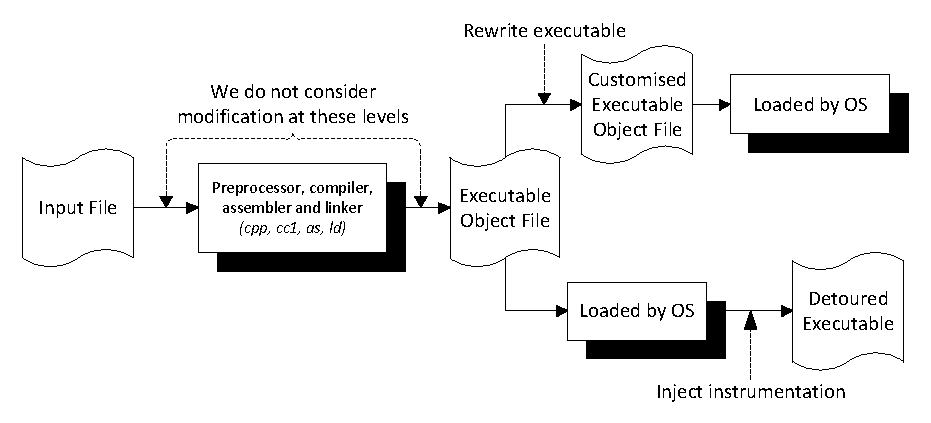
\includegraphics[viewport=21 566 448 757]{Detouring_Options.pdf}
 \caption[Detouring Options]{Our options for inserting instrumentation code. Since we only have access to the executable in its final compiled form, we focus solely on binary level options.}
\end{figure}

\subsubsection{Executable Editing vs Runtime Detouring}

Also known as static code annotation\cite{static_code_annotation}, executable editing is seen as the most convenient to the end user because a single command can be applied to one executable file generating a customised program which can be easily distributed. In comparison, with runtime detouring we are often required to set up a specific runtime environment which might be difficult to use and deploy. In the cases where the production system is on a cloud system such as EC2, this means reconfiguring many environments.

However, the attractiveness of executable editing is reduced when considering the complexity of implementation. Despite being conceptually trivial, executable editing is complex to implement in practice because of architectural and system-specific details. This increases the time and effort required to produce such a tool. Furthermore, at the binary level, symbol-table information is often incomplete and significant analysis must be performed to properly relocate code and data\cite{rewriting_executable_files}.

\subsubsection{Executable Editing}

Conceptually, binary rewriting generally entails a standardised procedure:

\begin{enumerate}
 \item \textbf{Code discovery/analysis} - During this stage, a tool typically analyses the binary and provides an interface to enumerate routines and code blocks which can be split into their constituent instructions. The tool must be able to accurately distinguish between code and data in this case.
\item \textbf{Insertion of instrumentation code} - The insertion stage tends to happen separately and allows insertion/deletion of instructions from the structures discovered in the first stage. It is standard for a tool to allow both the modification of the original binary as well as to provide an option to create a new customised one.
\end{enumerate}

\paragraph{Register Scavenging}

When inserting code to an executable, it is critical not to break the original code by overwriting data or otherwise functionally changing the program in an unintended way. At the assembly language level, this means it is important not to overwrite registers that are in use. Register scavenging uses control flow analysis to provide information about unused registers at any point in a basic block\cite{qpt}. If unused registers can not be found, a last resort is to \emph{push} and \emph{pop} registers to temporarily evict them so they are available for usage.

\paragraph{ELF}

(Executable and Linkable Format) is the file format for executables, object code and shared libraries on Unix-based systems. \emph{libelf} is a library used to directly read, modify and create ELF files in an architecture-independent way. It would be ideal to abstract away from the ELF file format since it is so specific and low-level.

\paragraph{BFD}

(Binary File Descriptor) is a package which allows applications to use the same routines to operate on object files whatever the object file format\cite{bfd}. BFD encapsulates many file formats over many different architectures and presents a common view of them and then provides a unified API to this view. As we will see, some existing Linux binary rewriters build directly over the ELF file format and perform modification through libelf. Although this is a lightweight alternative to BFD, it is undesirable because it locks the code down to a specific file format. Whilst the abstractions BFD provide limit functionality in comparison to dealing with the specific file format directly, it makes it powerful for this precise reason, allowing any library built on top of it to effortlessly and automatically handle differences between and hence support the various formats.

\subsubsection{Runtime Implementation Approaches}

To perform detouring at runtime but achieve the same effect as if it was performed statically, the target must be forced to execute special code as part of its startup - before it starts execution. The purpose of this code is to ensure the instrumentation code is mapped into the target's address space and also to either perform the placement of the detours or implement some system which can perform the detouring dynamically. We now examine different implementation approaches employed by existing tools and research projects.

\paragraph{Shared Library and Position-Independent Code}

Once we have the ability to execute arbitrary code in a target, the placing of the detours at runtime is a trivial matter. The issue we face is how to insert the instrumentation code in the first place and also how to override execution to make sure our special code is run before anything else. One method is to patch the entry point of the target to dynamically load a shared library containing the instrumentation code through the \texttt{dl} interface with functions such as \texttt{dlopen}.  Whilst this does require static insertion of the bootstrapping code, the amount of work required is minimal. One further advantage is that the shared library will already have been compiled to have position-independent code, which means that the Linux loader deals with all the linking of our extra library, something we are required to perform manually with binary rewriting.

GCC conveniently provides a constructor attribute, \texttt{\mbox{void \_\_attribute\_\_ ((constructor))}} which can be used to specify a function which is invoked upon loading of the shared library. With this approach, the constructor would set up the hooks before the main program starts executing:

\begin{lstlisting}[language=C,caption={This example would be compiled as a shared library}]
void init(void) __attribute__ ((constructor));

void init(void)
{
   /*
    * This function is invoked as soon as the library 
    * is loaded. In a dynamic implementation, we would
    * place the code to perform the detours here.
    */
}
\end{lstlisting}

An alternative to patching the executable's entry point to load the bootstrapping library is to use the \texttt{LD\_PRELOAD} environment variable which adjusts the runtime linking process by preloading a shared library into an arbitrary process. Unfortunately, \texttt{LD\_PRELOAD} can be subverted by the application which means this option is unreliable.

\paragraph{Exception Handlers}

Methods used for general debugging often require the breaking or redirection of code flow. One common form of this is breakpointing which comes in two flavours - hardware and software breakpoints. The breakpoint suspends execution before some given instruction is executed and the programmer inspects the program context at that point. As well as inspecting the context, it is possible to modify it, or more specifically the instruction pointer. In the context of a detouring implementation, software breakpoints are often used by replacing instructions with the \texttt{int 3} opcode which when executed triggers an interrupt handler. The interrupt handler can be overridden to modify the EIP/RIP register\cite{fast_breakpoints, profiling_unix, kprobes}.

Similarly, the access protection of memory pages can be changed to become non-executable pages so each access invokes a global exception handler. As with breakpoint trapping, the ability to trap each instruction implies the capability to redirect code flow. Although this approach is interesting, the overhead is too large to be useful in practice.
\section{Related Work}

Given the limited amount of related work in the Linux arena, it is well worth it to look at work that has been done for other operating systems as it may influence our final design. The related work will also act as case studies of current techniques used for detouring.

\subsection{Microsoft Detours}

\textbf{Detours} is a mature proprietary Microsoft library for the Windows operating system which provides functionality for the interception of arbitrary Win32 functions\cite{detours_microsoft_research}. The library only allows detours to be inserted at execution time by modifying memory as with the dynamic approach described earlier. The rationale given for this is that it facilitates interception at a very fine granularity allowing detouring of one running instance of an application whilst another instance of the original application runs alongside. However, this is not an exclusive feature of dynamic detouring since executable editing tools often allow the creation of a new executable.

When Detours was initially released, it introduced trampolining, a feature not seen with other detouring packages released at the time. Other features supplied by Detours are Windows-specific such as the ability to edit import tables of binaries. Detours instruments code extremely efficiently with benchmarks placing interception overheads at less than 400ns on the 200MHz processors the library was initially tested on. Another advantage over binary rewriters is size, with Detours adding less than 18KB to an instrumentation package. However, this comes at the cost of an inability to insert code between instructions or basic blocks. Binary rewriters can typically insert instrumentation arbitrarily by performing sophisticated code analysis with techniques such as register scavenging. On the other hand, Detours relies on matching calling conventions to properly preserve register values at the function level. For example, \textbf{stdcall} designates \textbf{eax}, \textbf{ecx} and \textbf{edx} for use within a function and hence these registers are trashable by instrumentation code. This method would not be appropriate for our case since we require modification at the basic block level where looking solely at the call convention would not help determine free registers.

\subsubsection{Advantages and Disadvantages}

Detours is a lightweight library with a distinctly clean API which has no doubt contributed to its success on the Windows platform. The library is written such that a user can make good use of it with only a superficial understanding of Windows internals. Even though Detours is only available for Windows, we can likely borrow from or at least be influenced by its API if we implement dynamic detouring. From a technical level, Detours works in a similar way to the \emph{LD\_PRELOAD} method we described previously. It performs a very limited amount of static manipulation on the target binary's import section to have it load the DLL (Windows' equivalent of a shared library). Since the details of editing the import section are Windows-specific, we shall not go into it further. However, later we will see the same technique employed on the Linux platform by LEEL.

\subsection{EEL}

\textbf{EEL} (Executable Editing Library) is a library for building tools to analyze and modify compiled executable programs on SPARC systems\cite{eel}. EEL works by removing existing instructions and adding foreign code that observes or modifies the original program's execution. Binary rewriting is non-trivial so it is worth it for us to discuss in more detail the intricacies of this technique. The tool provides five major conceptual abstractions in the form of C++ class hierarchies:

\begin{enumerate}
 \item \textbf{Executable} - This is the top-level abstraction which represents any container of executable code, regardless of the specific format.
 \item \textbf{Routine} - Executables contain many routines, which are discovered by the library through static code analysis.
 \item \textbf{CFG (Control-Flow Graphs)} - A CFG is a directed graph with nodes as basic blocks and edges representing control flow between these blocks. The CFG is also generated through static control-flow and data-flow analysis.
 \item \textbf{Instruction} - Basic blocks are composed of these machine-independent descriptions of opcodes. Each instruction object holds intimate information about what registers is reads/writes, which aids data-flow analysis.
 \item \textbf{Snippet} - Snippets encapsulate the machine-specific foreign code that is to be added (instrumentation code). Snippets also take responsibility for register allocation through the use of register scavenging. Snippets often need to be written in assembly language although the authors argue this is not a drawback because the code is usually short and carefully written for efficiency. Useful work is done by separately inserting user defined routines which the snippets call out to.
\end{enumerate}

The abstractions EEL provide are not merely there to hide the complex and low-level implementation details but more so to provide machine-independence. All static analysis performed by the library is completely machine-independent and is supported by requiring every implementation of the EEL library to contain a separate backend-frontend mapping of architecture-specific instructions to EEL's own representation. Theoretically, the library could be ported to any architecture if the appropriate translations were made from EEL instructions to the machine-specific instructions. However, EEL was originally written for RISC instruction sets such as SPARC and MIPS. For this reason, CISC instructions are difficult to synthesize effectively in terms of EEL instructions. For example, string-manipulation instructions such as \textbf{movs}, \textbf{scas}, etc. do not interact with registers in a trivial way. It is not ideal to model the dynamic behaviour and internal control flow of x86 CISC instructions such as these against classic RISC instructions. One approach is to model a CISC instruction as multiple RISC instructions\cite{intermodule_code_optimization}, but this is inconvenient, complex and exposes underlying implementation details thereby breaking abstractions.

Despite the focus on portability, EEL still has architecture-specific details even within its instruction class due to the non-generic nature of some of its target instruction sets. An example of this is representation for delayed branching which is inherent to SPARC but completely absent in the x86 instruction sets. Details such as these unnecessarily add extra complexity to the final library if we were to port it to x86-32 and x86-64.

The portability in itself is a double-edged sword since EEL has catered for it to such an extent that the library and API has become clunky and complicated in comparison to libraries such as Detours. The last update to the source of EEL was well over a decade ago and it is likely the code is now too outdated to be of feasible use to us. Furthermore, the library is already far too bulky to consider extending and this is driven home by the unacceptable size markup when adding even basic instrumentation code. A simple program written in C with a size of 8KB is bloated to 350KB after insertion of a minimal amount of instrumentation code which simply instruments all routines to print their names\cite{leel}. The reason for this is that EEL inserts code from an object file containing the new routines. Since it is unknown whether these routines call sub-routines, the whole object file is inserted. One of the requirements for our tool is that it must be lightweight and have minimal impact to performance so we must avoid this problem in our final solution.

\subsubsection{Advantages and Disadvantages}

EEL presents a complete system for executable editing even though it is too vast to be of direct use to us. Despite this, it is interesting to consider the concept of the machine-independent representation which adds a layer of abstraction above machine-specific opcodes and allows the library to be ported to multiple architectures (previous versions also ran on MIPS, but the most recent version works only for SPARC). Some of the more novel design decisions such as the use of CFGs and the use of an abstraction layer are certainly tempting features to include in our implementation if we opt for executable editing. However, we are only considering Linux x86-32 and x86-64, so adding an extra layer of abstraction may not be necessary since the two instruction sets do not differ greatly. Instead, a more appropriate option as an abstraction layer might be to build on top of the BFD library.

\subsection{LEEL}

\textbf{LEEL} (Linux Executable Editing Library) is an executable editing library for Linux systems running on Intel x86-32 processors\cite{leel}. The project was motivated by EEL and the workflow of tools using both libraries are similar. LEEL identifies shortcomings of the original EEL library and addresses them by adapting a new design. The final product closely resembles EEL from a functional aspect so we will discuss mainly the additional features offered by LEEL\footnote{It should be noted that the similarities and differences discussed are concerning LEEL acting upon executables. It is outside the scope of this project to consider editing relocatable object files and shared libraries.}:

\begin{enumerate}
 \item \textbf{Editing of multiple formats} - LEEL supports editing of executables, relocatable object files and shared libraries.
 \item \textbf{Insertion of user defined routines} - Insertion of user defined routines differs significantly to what we have seen with EEL. It is useful to recall that EEL inserted user defined routines by requiring them to be supplied in an object file which was then inserted into the target. Similarly, LEEL recommends users do most of their processing in an external routine instead of in the snippet itself. However, instead of defining the external routines in an object file, LEEL requires the routines to be contained in a shared library. As we will see later, this is a similar approach to that taken by Etch.
 \item \textbf{Insertion of snippets to CFG} - Snippets in EEL need to be written as small chunks of assembly, but LEEL expects most work to be done in external routines. With this expectation, it simply exposes an API which allow users to generate the assembly code for common tasks such as calling an external routine.
 \item \textbf{Lightweight} - One of the problems with EEL was the huge file bloat after the injection of user-defined routines. Files generated by LEEL have a small overhead in comparison (a sample program with an original size of 11KB is increased to less than 17KB). The problem was solved by having users compile their routines into a shared library and calling out to these routines from instrumented code. A side effect of this is that the development of this shared library and the creation of the snippets can be performed independently as long as function names and signatures are agreed upon. Furthermore, after the new executable is generated, the shared library can be continually updated without requiring further executable editing as long as it continues to adhere to the mutually accepted function names and signatures.
\end{enumerate}

\begin{figure}[H]
 \centering
 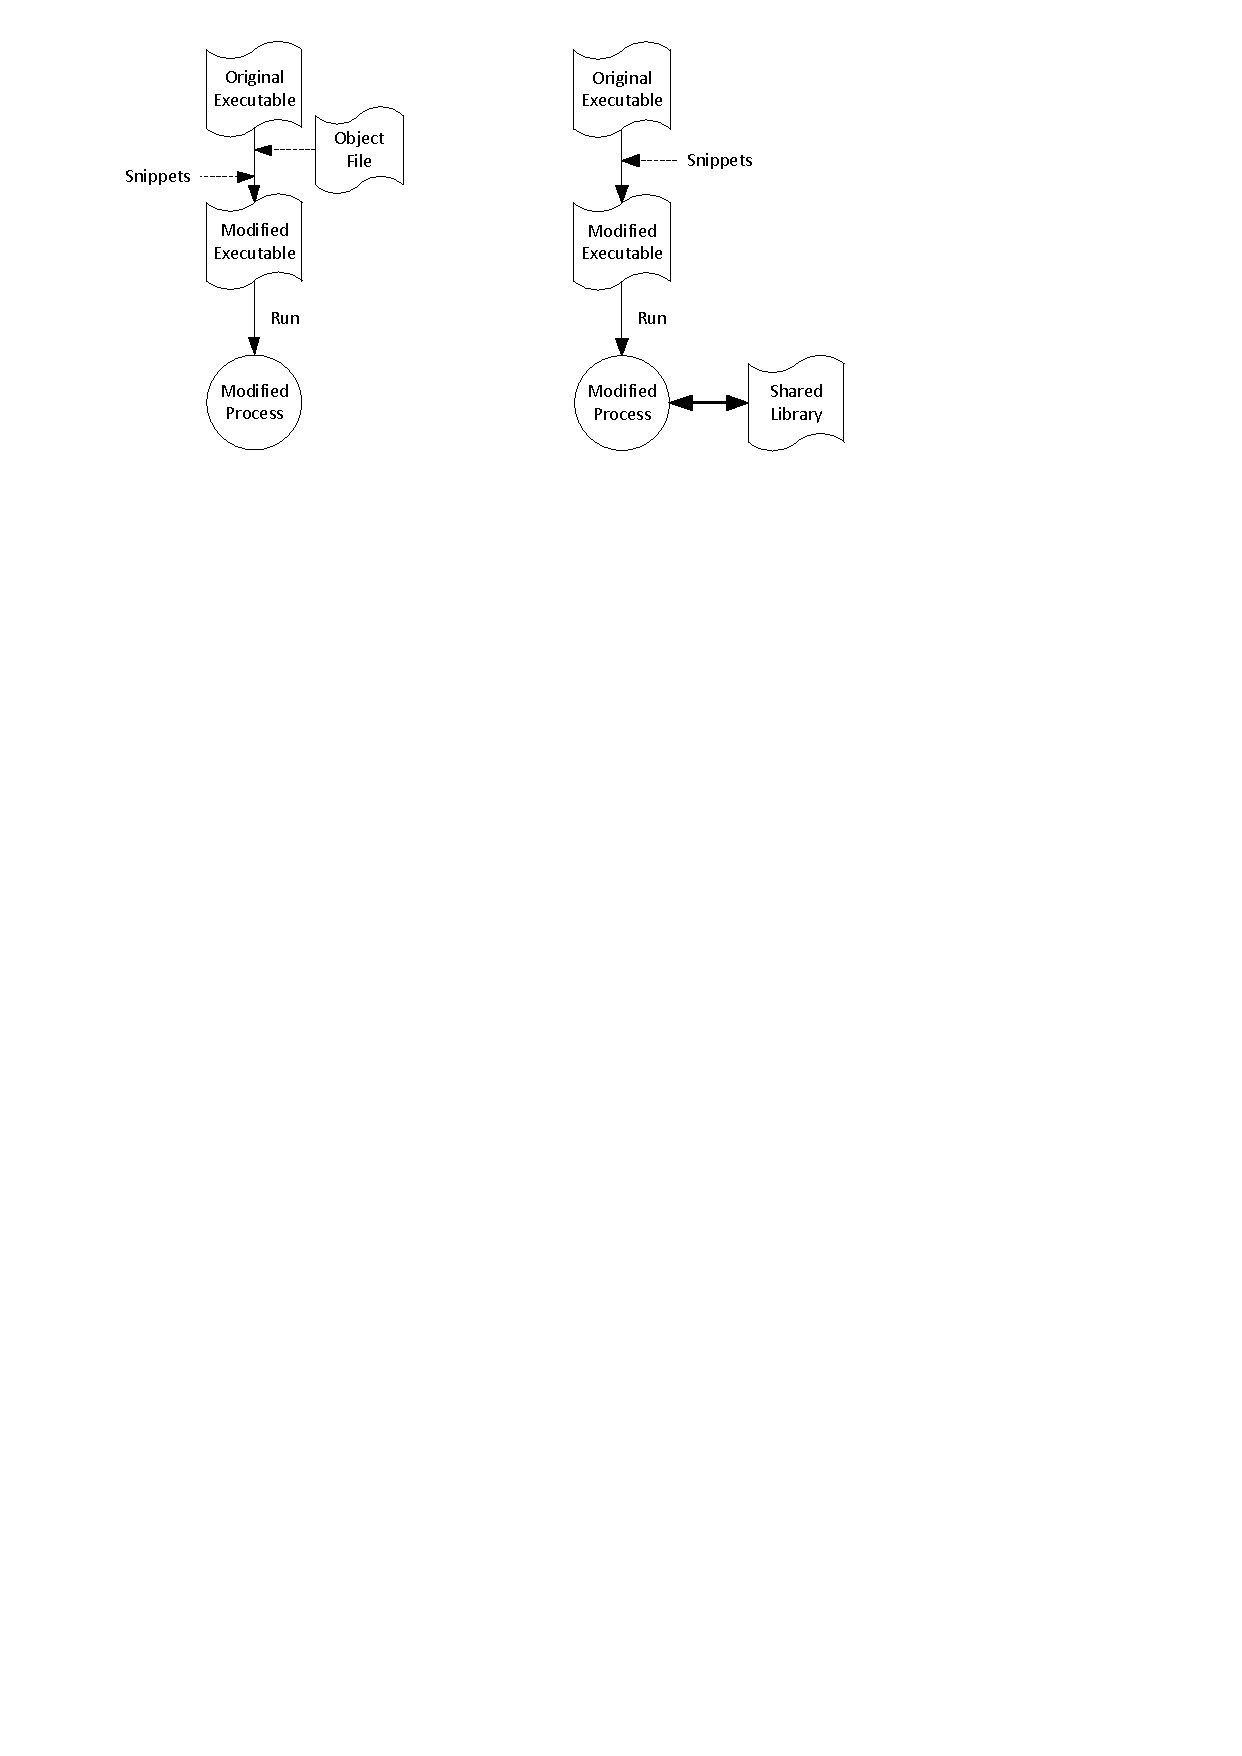
\includegraphics[viewport=60 624 406 825]{LEEL_vs_EEL.pdf}
 \caption[LEEL vs EEL]{The left-hand side shows an executable being modified by EEL. An object file is inserted containing user-defined routines. Snippets allow the original code to be modified to make use of the new routines. The right-hand side shows the same process via LEEL. Snippets are inserted to make use of external routines in a shared library. The shared library is made available at runtime.}
\end{figure}

The only major stage we did not elaborate on is the static analysis stage of LEEL. As with EEL, the library must perform duties before modification of code occurs. Namely, routines need to be identified and a CFG generated - code flow analysis. However, it is uninteresting to delve deep into this since the process does not differ substantially from EEL. The main difference is in the data flow analysis, which LEEL does not perform at all. The justification for this is that with EEL, snippets are expected to be highly optimized and carefully written and this is why register scavenging is performed (which requires data flow analysis). With LEEL, the focus is less on the snippets and more on the external routines so the code is simply wrapped in \textbf{PUSHAD}/\textbf{POPAD} to automatically save and restore the registers. Register scavenging is also less valuable on the Intel processor because of the relatively few number of registers in comparison to SPARC and is not worth the extra complexity of analysis attributed to a more complex instruction set. One midway alternative that LEEL could have used is matching call conventions as part of the agreed external routine signatures, which would inherently allow the snippet to know which registers were used in the external routine. This is the technique used by Detours.

\subsubsection{Advantages and Disadvantages}

While LEEL offers many desirable features, it has a fundamental abstraction design which is unsuitable for us. The library achieves this by building on top of the ELF library. This was a deliberate design decision and reflects one of the key differences in the aims of the two libraries. Whereas one of EEL's main focuses was portability, LEEL intended only to achieve portability to Win32. Since there exists no backend port of BFD to Win32, this resulted in the decision to work directly with ELF instead. Porting LEEL to use BFD as an abstraction layer is infeasible. It would require almost entirely reprogramming the backend and it would take a lot of effort to avoid breaking the support for the specific cases of relocatable object files and shared libraries. In fact, even porting the library to support x86-64 would be very tough because of the tight coupling against the x86-32 instruction set. As a minor point, LEEL also does not support trampolining although this would not be overly difficult to implement. Despite these drawbacks, LEEL presents good solutions to the same drawbacks we identified with the EEL library.

Executable editing is a complicated process and both EEL and LEEL recognise this by demonstrating huge efforts to minimize the amount of code instrumented directly to the target (snippets) by allowing the compilation of the majority of the code (user defined routines) to be performed separately by the compiler. This code is then integrated at two different stages, either by merging the object file with the executable statically (EEL) or merging the code in the form of a shared library at runtime (LEEL). Overall, LEEL can get away with performing less binary rewriting by shifting the focus to the external routines, but the price for this is that it needs to deal with the additional complexities of:

\begin{enumerate}
 \item \textbf{Modifying the executable to use the shared library} - The target has to be modified to act as if it had originally been dynamically linked to the shared library. This process involves an intimate understanding of the file format.
 \item \textbf{Calling of external routines from snippets} - The snippets must deal with the complexities of interacting with the position independent code of the shared library, where the absolute address of the external routines is not known statically.
\end{enumerate}

\subsection{Etch}

\textbf{Etch} is a general-purpose tool for rewriting arbitrary Win32/x86 binaries without requiring source code\cite{etch}. Binary rewriting under the Win32 environment poses complications which are not present in UNIX-based environments due to system-specific features. It is outside the scope of this project to discuss such challenges, so we shall omit them from this report and focus on the higher level concepts of Etch.

Unlike EEL, Etch weaves the instrumentation phase tightly with the code discovery phase, but uses a separate analysis stage. Etch defines two phases: an instrumentation phase and an analysis phase. The instrumentation phase represents the insertion of instrumentation and modification of the program and the analysis stage represents the program at runtime. A tool created using Etch is similarly split into an instrumentation module and an analysis module with the analysis module being loaded with the executable at runtime. An approximation of the workflow is:

\begin{enumerate}
 \item \textbf{Code Discovery} - Etch performs static code analysis to discover the components of the program. \emph{Figure \ref{fig:EtchHierarchy}} illustrates how Etch views the program hierarchy.
 \item \textbf{Callback} - The instrumentation module supplies a callback which Etch calls upon discovery of each component. Each invocation of the callback provides an opportunity to insert instrumentation or modify the executable. This modification can happen at the instruction, basic block or procedural level. Inserted instructions may include calls to procedures in the analysis module.
 \item \textbf{Executable Generation} - The complete traversal of the executable concludes the instrumentation stage and a new executable is generated.
 \item \textbf{Running the Executable} - The executable is run alongside the analysis module. Etch provides a hook providing notification to the analysis module of program completion. The module can then optionally run some analysis routines based on data collected during execution.
\end{enumerate}

\begin{figure}[H]
\Tree[.Program [.Module [.Procedure [.{Basic Block} Instruction {\ldots} ] {\ldots} ].{Procedure}
      {\ldots} ].Module {\ldots} ]
\caption{Etch views a program as a collection of modules. Each module contains procedures, which are composed of basic blocks which in turn are composed of instructions.}
\label{fig:EtchHierarchy}
\end{figure}

Etch provides additional features which are less related to executable editing. For example, it provides facilities to rewrite an executable in order to improve its performance by reordering instructions to optimize code layout to take advantage of spatial and temporal locality. This is a relatively complex example and application of data flow analysis alongside executable editing.

\subsubsection{Advantages and Disadvantages}

Etch presents a vastly different front-end interface compared to EEL, working less directly through the callback system established in the instrumentation module. Since Etch is not an open source project (nor even publicly available), to some extent, we can only speculate about the underlying implementation of the tool. However, it would appear that the separation of `instrumentation' and `analysis' simplifies the task of the editor slightly. By mapping the analysis module in at runtime, calls from the instrumentation can be dynamic which lightens the workload of the executable editing part of the tool by decreasing the amount of code that needs to be injected statically. Essentially, the task of code injection is partially delegated to the OS loader to be performed at runtime, which makes Etch more of a static/dynamic hybrid rather than a strict static binary rewriter.

Aside from the technical ramifications, the separation of the two duties reflects a different approach to the creation of a tool through Etch. It allows a user to treat the analysis module as a library and also decouples the instrumentation from the logic of analysing the data gleaned at runtime. In a way, this is more natural than the approach taken with EEL which tends to focus on the injection of small and optimized snippets of code.

\subsection{ELFsh}

\textbf{ELFsh} is an interactive, modular, and scriptable ELF machine for static binary instrumentation of executable files, shared libraries and relocatable ELF objects\cite{elfsh}. ELFsh differs from most other implementations in that it does not come in the form of a library nor does it provide a programmatic interface other than in the form of a scriptable command-line. The main way to use ELFsh is interactively through the command prompt. The tool provides access to many low-level features such as reading and writing of ELF sections and symbol tables. However these features are not only file-format specific, but also do not directly provide useful functions to an end-user and should be abstracted in our tool. The reason these features are available in ELFsh from the user-level is mainly because of the implementation approach taken. From a high-level, ELFsh provides the following features:

\begin{enumerate}
 \item \textbf{Injection of instrumentation} - The instrumentation must be in the form of an object file and is added into the target as if the binary has not been linked yet. Internally, this works by adding a library dependence to the main object\cite{cerberus_elf}.
 \item \textbf{Function redirection} - By exploiting the way that dynamically linked function calls are resolved, existing procedures can be hijacked. When resolving symbols, the runtime linker iterates over a \emph{link\_map} list and resolves each symbol to an absolute runtime address where the function is mapped. By forcing some symbols to be resolved in priority, ELFsh is able to control the procedures to which symbols resolve to. ELFsh does not provide convenient access to the original function. Instead, the common practice to access it is to call \texttt{dlopen} and \texttt{dlsym} in the hook function. This allows a function address to be resolved at runtime based off a module and function name.

\end{enumerate}

\subsubsection{Advantages and Disadvantages}

ELFsh demonstrates less conventional techniques for the binary rewriting process, which is due to its birth in the reverse engineering scene. For the most part, the tool is able to avoid dealing with concepts such as static code analysis by relying on pre-existing analysis from the user. For example, it provides no function to enumerate procedures so the parameters to \texttt{dlopen} and \texttt{dlsym} would have to be determined beforehand at the compile-time of the instrumentation object file. The tool is able to discover such information interactively but the lack of a proper programmatic interface makes the process much more manual. The tool is unsuitable for us for various other reasons:

\begin{enumerate}
 \item \textbf{Lack of abstraction layer} - As discussed earlier, one of our primary irks with ELFsh is the fact that it is built on top of libelf. This is exploited by using file-specific tricks to implement the features provided by the tool. The tool pays the price for this in portability, with ports requiring manual porting of the backend. The difficulty of this is evidenced in the fact that despite ports existing to other architectures, only the Intel version is fully featured.
 \item \textbf{Lack of granularity} - ELFsh lacks the granularity and control given with other binary editing tools. It does not allow the insertion of instrumentation at the instruction level, nor even at the basic block level. Another granularity related problem is that due to the nature of the injection (entire object file injected), the tool faces similar size markup issues as seen with EEL.
 \item \textbf{Development state} - ELFsh is an old project that is no longer maintained or developed.
\end{enumerate}

One concept we can take away from ELFsh is the scriptable command-line. Even though we want to create a library, it would be nice to be able to operate our tool through a command-line also.

\subsection{Pin/DynamoRIO}

\emph{Pin} and \emph{DynamoRIO} are two tools which perform run-time binary instrumentation of Linux and Windows applications\cite{pin,pin_windows,dynamorio}. The two tools are completely separate but due to the similarities of their implementation they have been grouped together here. We will talk about Pin, but the concepts are applicable to both tools unless explicitly stated.

Pin does not make any static modifications to the executable. Instead, it uses \emph{dynamic recompilation} to run the target in a process-level virtual machine which intercepts execution at the entry point and injects a runtime agent which performs the insertion of the instrumentation. 

Pin is used to create an architecture independent Pintool which can access architecture-specific details when necessary. The Pintools are written in C/C++ making them theoretically source compatible across different architectures. Pin is viewed as an efficient solution compared to other runtime detouring implementations because of its use of just-in-time (JIT) compiling to insert and optimize code.

\subsubsection{Advantages and Disadvantages}

The advanced process-level virtual machine Pin utilizes requires the distribution of a substantial environment so is not quite suitable for us. However, interception from this level allows for a high level of observability which is usually difficult to obtain. Whereas the tools we have looked at so far operate mostly at the instruction, basic block and procedural level, Pin allows higher level abstractions to be observed. For example, instrumentation can be notified upon events such as loading/unloading of shared libraries and creation/end of threads. It is possible to reproduce these effects with regular tools by detouring system library functions but this convenience and ease of use is one of Pin's selling points. If we have time, it would be good to mimic this concept of moving more responsibility from the user to the library.

Pin takes full advantage of the flexibility offered by dynamic detouring presenting features such as process attaching and detaching. Pin suffers from the overhead inferred from runtime attachment, but makes up for it with its powerful JIT compiler. Firstly, by performing code discovery at runtime, Pin is able to gather more comprehensive information about the program compared to using static control flow analysis. This extra information allows the tool to perform optimizations on instrumentation which previously had to be done by the user. Secondly, the JIT instruments code on the fly by taking the native executable as input and intercepting its execution, generating new code from it (which is cached) and transferring the target's execution to the generated sequence. Instrumentation can easily be inserted during the translation phase. This process essentially optimizes the code on the fly with the further advantage that the system can reflect the target's runtime environment accurately reducing any effects on the original program's behaviour.

Pin was designed with observation in mind, rather than modification. It can modify the behaviour of the executable by modifying registers and memory but its ability to do so is more limited than some of the other tools we have looked at. In a way, Pin has taken the typical inspections that users might make with regular detouring tools and made these accessible features as part of its API.

\subsection{IDA Pro}

\emph{IDA Pro} is a popular commercial disassembler supporting a large variety of architectures and operating systems\cite{ida,stripped_binary}. The focus with IDA Pro is not on the instrumentation phase, but rather on the automatic code analysis that it performs. The tool is able perform instrumentation, but since it does not present anything substantially different to what we have already seen, we shall draw our comparisons about its ability to perform static analysis.

\subsubsection{Advantages and Disadvantages}

As with all static binary rewriters, IDA Pro faces the problem of discovering functions that are only reachable through indirect control transfer. What is interesting in this case is not what IDA Pro provides, but what it lacks and how it contrasts with solutions provided by other tools.

IDA Pro and EEL both do not provide any support for discovery of functions that are reached via indirect calls. These functions become gaps in the code. LEEL approaches the problem by starting analysis from the program's entry point and recursively building a call graph (same so far). However, it provides two options to deal with the gaps\cite{leel}: either not to analyze them at all or assume that the first byte of a gap is the starting address of a function. It can be argued that this provides two extremes, providing either low code coverage or a high chance of incorrect analysis of non-code blocks as functions. Other tools such as RAD\cite{rad} take the more aggressive approach but use conservative heuristics to prevent false positives such as only analysing blocks if it starts with a known prologue. If we perform static analysis, we will need to take these methods into account and select one appropriately.

\subsection{Others}

There exist various other noteworthy libraries and tools which either perform detouring or make use of it including \emph{Valgrind}, \emph{IDtrace}, \emph{radare2}, \emph{qpt}, \emph{ATOM} and \emph{pixie}\cite{valgrind,IDtrace,radare2,qpt,atom,qpt_pixie}. However these tools do not introduce significant concepts or techniques interesting to us that we have not already seen so we shall not be covering them in further depth.
\chapter{Design}\label{chap:Design}

This section goes over the initial design for the solution we present. Any major deviations from this design are noted in Chapter~\ref{chap:Implementation}. To make design decisions, we re-evaluate the functional requirements taking into account the techniques gleaned and the lessons learnt from Background and Related Work

\section{Static vs Dynamic}

The first and largest choice faced is whether to use dynamic or static detouring for our library. After deciding this, we can evaluate the available implementation options.

Even though implementing detouring at runtime offers advantages such as flexibility and ease of development, it was ruled out as an option because we did not find a dynamic method which does not compromise \emph{(F6)}. That is, all the runtime methods we have looked at require some form of environment, whether this is through the distribution of a shared library, process-level virtual machine or otherwise. Since a dynamic solution is infeasible, we can narrow the scope of the solution to the various static binary rewriting approaches.

\section{Proposed Workflow}

In order to make further design decisions, we take a top-down design approach. We first define the expected workflow with a tool created with our library. After this is decided, we can fledge out the design details for the implementation of each stage of this workflow. Figure~\ref{fig:Workflow} illustrates the proposed workflow of our library according to the exemplary model described in Chapter~\ref{chap:Introduction}.

.........
approach borrows from the workflow of eel. the similarity lies in the fact that we inject an object file.

however, because we are only targeting x86-32 and x86-64, we can make some improvements, particularly in terms of expressibility. eel caters for many architectures and for this reason, requires users to directly write small chunks of assembly which will be patched into the executable. while it is nice to expose such functionality, it would be nice to abstract away entirely from assembly language. since we are only targeting two architectures, there is no need to expose such general functionality. even if we do choose to expose it, we can do better by providing a rich API for detouring and trampolining. since this is the main focus. it is important to note that the main focus of the library is detouring, so having a more specific api which is less cumbersome may well be preferable to having a very general one that allows everything to be done.

another difference from eel is that we should try to address the problem of overhead in object injection. to recap, the reason for the overhead is that when an object is inserted, all its dependencies are also recursively inserted, which are required to be statically linked. the problem with this is that if the object file is linked against libc, then a copy of the entire libc library will be pulled into the binary upon injection 
theoretically, this should not be necessary. that is, if the target is already linked against libc (whether dynamically or statically), it is redundant to pull in an extra copy of the library. we should not be limited by the fact that eel decided to take this route and instead we should investigate alternatives that allow object injection that does not duplicate dependencies.

\begin{figure}[H]
 \centering
 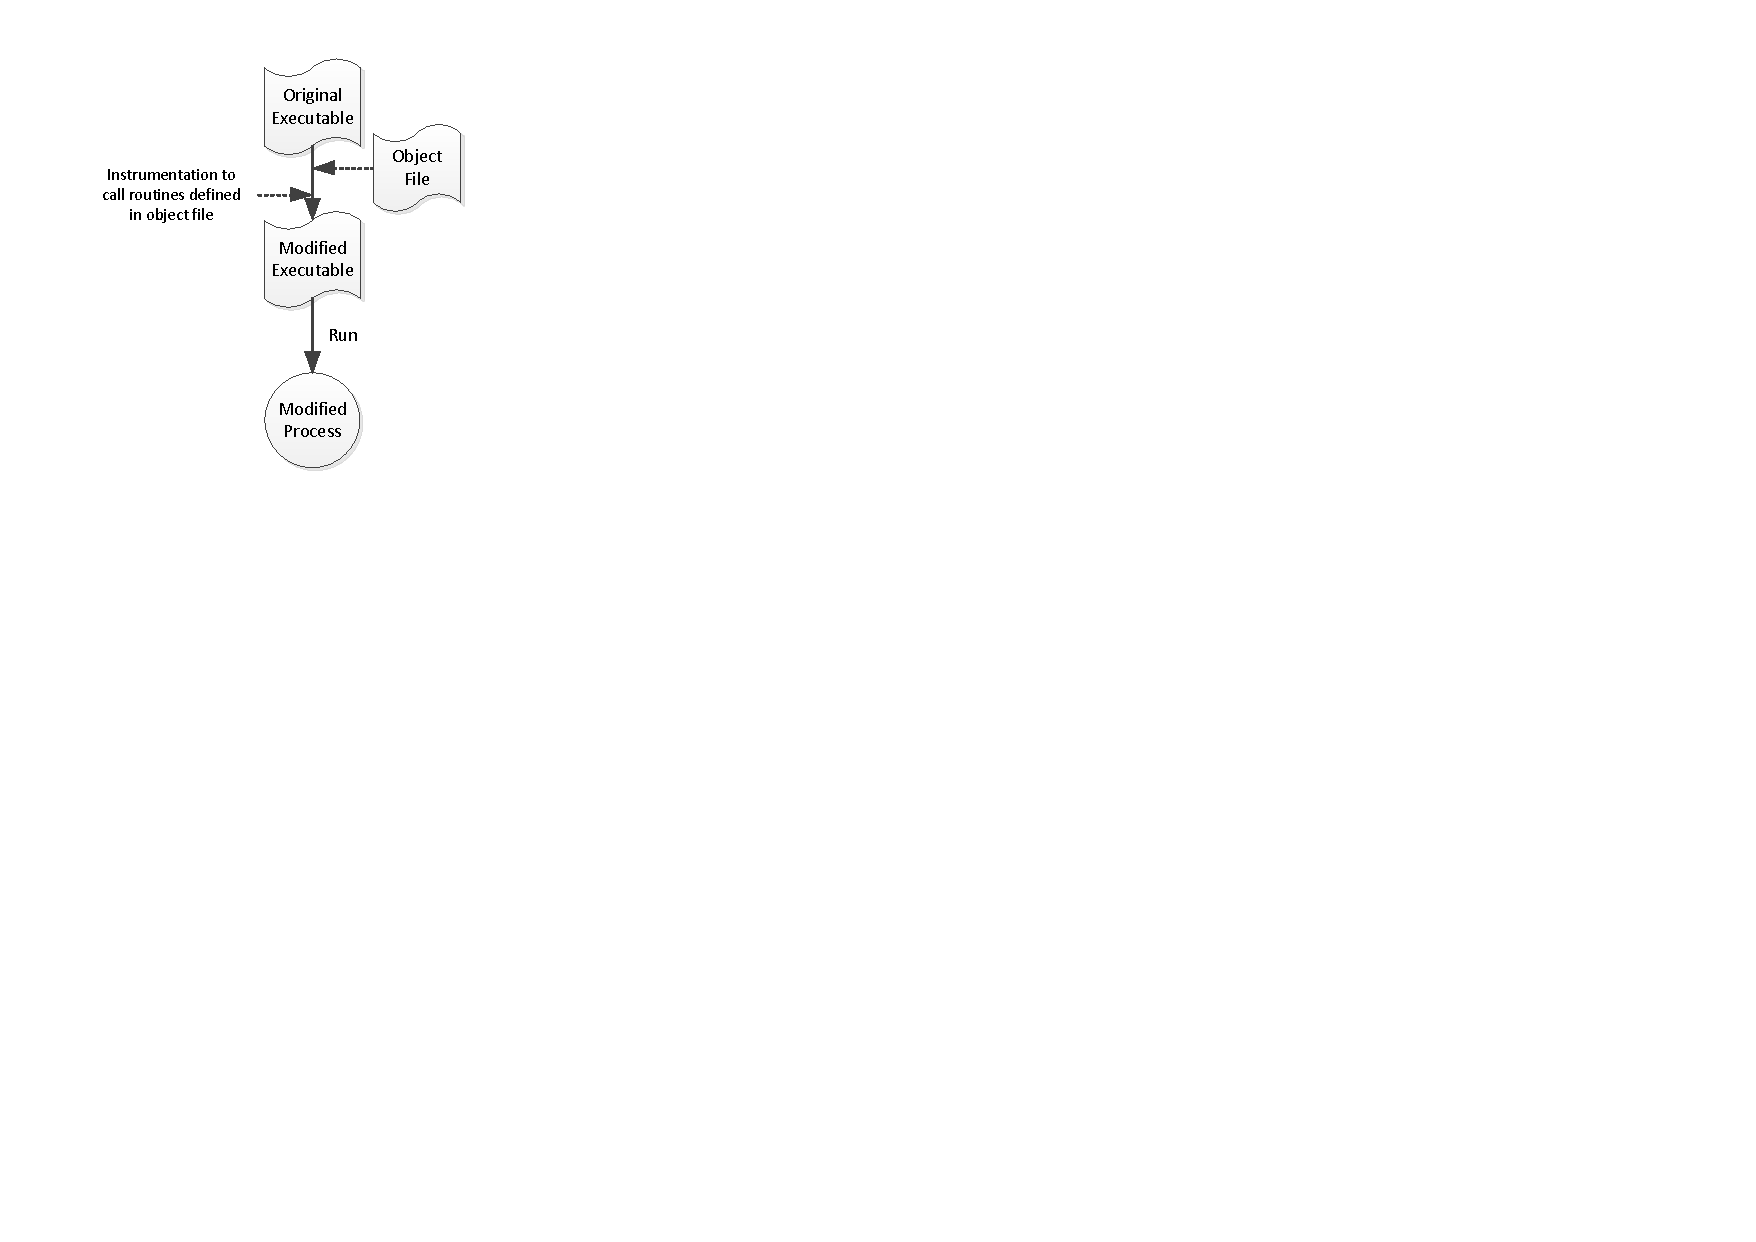
\includegraphics{Workflow.pdf}
 \caption[Hierarchy]{The proposed method for instrumentation. An object file containing user defined routines is optionally injected into the target binary. Using binary rewriting, the original code is then connected to the injected code.}
\label{fig:Workflow}
\end{figure}

from the proposed workflow, it can be seen that there are two distinct phases:

1. object injection which will take original binary + object => binary with user defined routines. satisfies f6.
2. binary rewriting to statically patch detours and trampolines into the binary which contains user defined routines. satisfies f1, f2, f3.

on top of this, we will add one more phase which is a binary analysis stage. we borrow the concept from Etch of having a code discovery stage. this will allow users to select what function or basic block they are going to detour/trampoline. this binary analysis should also produce the cfg that is required by \emph{(F4)} and \emph{(F5)}. in terms of \emph{(F7)}, it is an implicit implementation detail.

\section{Static Analysis Engine}

the static analysis engine corresponds to the binary analysis stage mentioned above. to re-iterate, the aims of the static analysis engine is to generate a cfg from a binary and expose an interface to it. the user then will iterate the discovered basic blocks and functions, choosing one to instrument. providing such functionality will require a disassembler engine.

\subsection{Disassembler Engine}

we could create our own disassembler engine, but that is unnecessary given the number of implementations already existing. it would be convenient to use a disassembler that can disassemble both x86-32 and x86-64. libopcodes is a natural choice because it is distributed as part of gnu binutils, which makes it readily available. furthermore, gnu binutils are ported to many platforms. this means that if it turns out in the future that we want to port our library to another architecture, it is likely we can reuse the disassembler engine. besides portability, one of the reasons using bfd is good is that it abstracts from libelf, which we want to avoid if possible \emph{(F7)}.

unfortunately, libopcodes has several shortcomings:
1. limited to disassembly of a single address (as opposed to disassembling a function, etc.)
2. designed to print to stream (not stored or analyzed)

libopcodes is likely to continue to be supported for the foreseeable future given that widely used binutils tools build on top of it. most notably, objdump. unfortunately, we are unable to make use of objdump because it does not support control-flow disassembly.

this means that in order to generate a cfg, we need to write our own code that generates one from single instructions. furthermore, we need to override the behaviour where it outputs to a stream. there already exists a library, libopdis, which wraps libopcodes to achieve exactly these core functionalities. however, we want a lightweight library so it is not optimal to build on top of libopdis. worse than this is the fact that libopcodes (like many disassemblers) only offers instruction information in terms of strings. string operation is inefficient and inconvenient so if we can find some solution which solves this problem, it would be good. in fact, even libopcodes returns strings when disassembling (it is meant to work with streams after all, so this makes sense). but this means libopcodes is a thin wrapper which should not be difficult to reproduce.

\section{Object File Injection}

...

\section{Static Patcher}

it is convenient that we are going to use bfd for the static analysis engine because it is also possible to write files through bfd. in fact, this is what several well known binutils tools do (e.g. objcopy and ld).

\section{Summary of Design}

We propose an implementation of executable editing which works on top of the BFD library. This makes adaquate use of existing functionality as required by \emph{(F7)}. BFD will work in conjunction with the libopcodes library to produce the control flow graph as required by \emph{(F4)} and \emph{(F5)}. To inject user-defined routines, we can take a similar approach to EEL and allow the user to specify an object file to be merged with the target binary.\todo{...} The next step would then be to find some mechanism by which procedural-level detouring can be achieved \emph{(F1)}, again through BFD. This is the first point at which we are modifying the target's code in any way. The technique used will have to be modified slightly to accommodate for the trampolining as required by \emph{(F2)}. Since the user defined functions are compiled separately to the target, they do not know what address to call for the trampoline so this is something we will have to deal with.
\chapter{Architecture}

This section discusses the architecture of libbind \todo{lib needs renaming} and presents its constituent components. The actual implementation will be covered separately so there may be minor inaccuracies and inconsistencies to keep things simple. Particularly, one key aspect of the library that should be noted is the support for both x86-32 and x86-64. While there is a high degree of overlap in code dealing with these architectures, the library delegates the work to architecture-specific sub-components for certain tasks such as instruction manipulation. Such differences will be addressed in Implementation\todo{make ref}, but ignored for now.

The following diagram illustrates the three main components of libbind:

\begin{figure}[H]
 \centering
 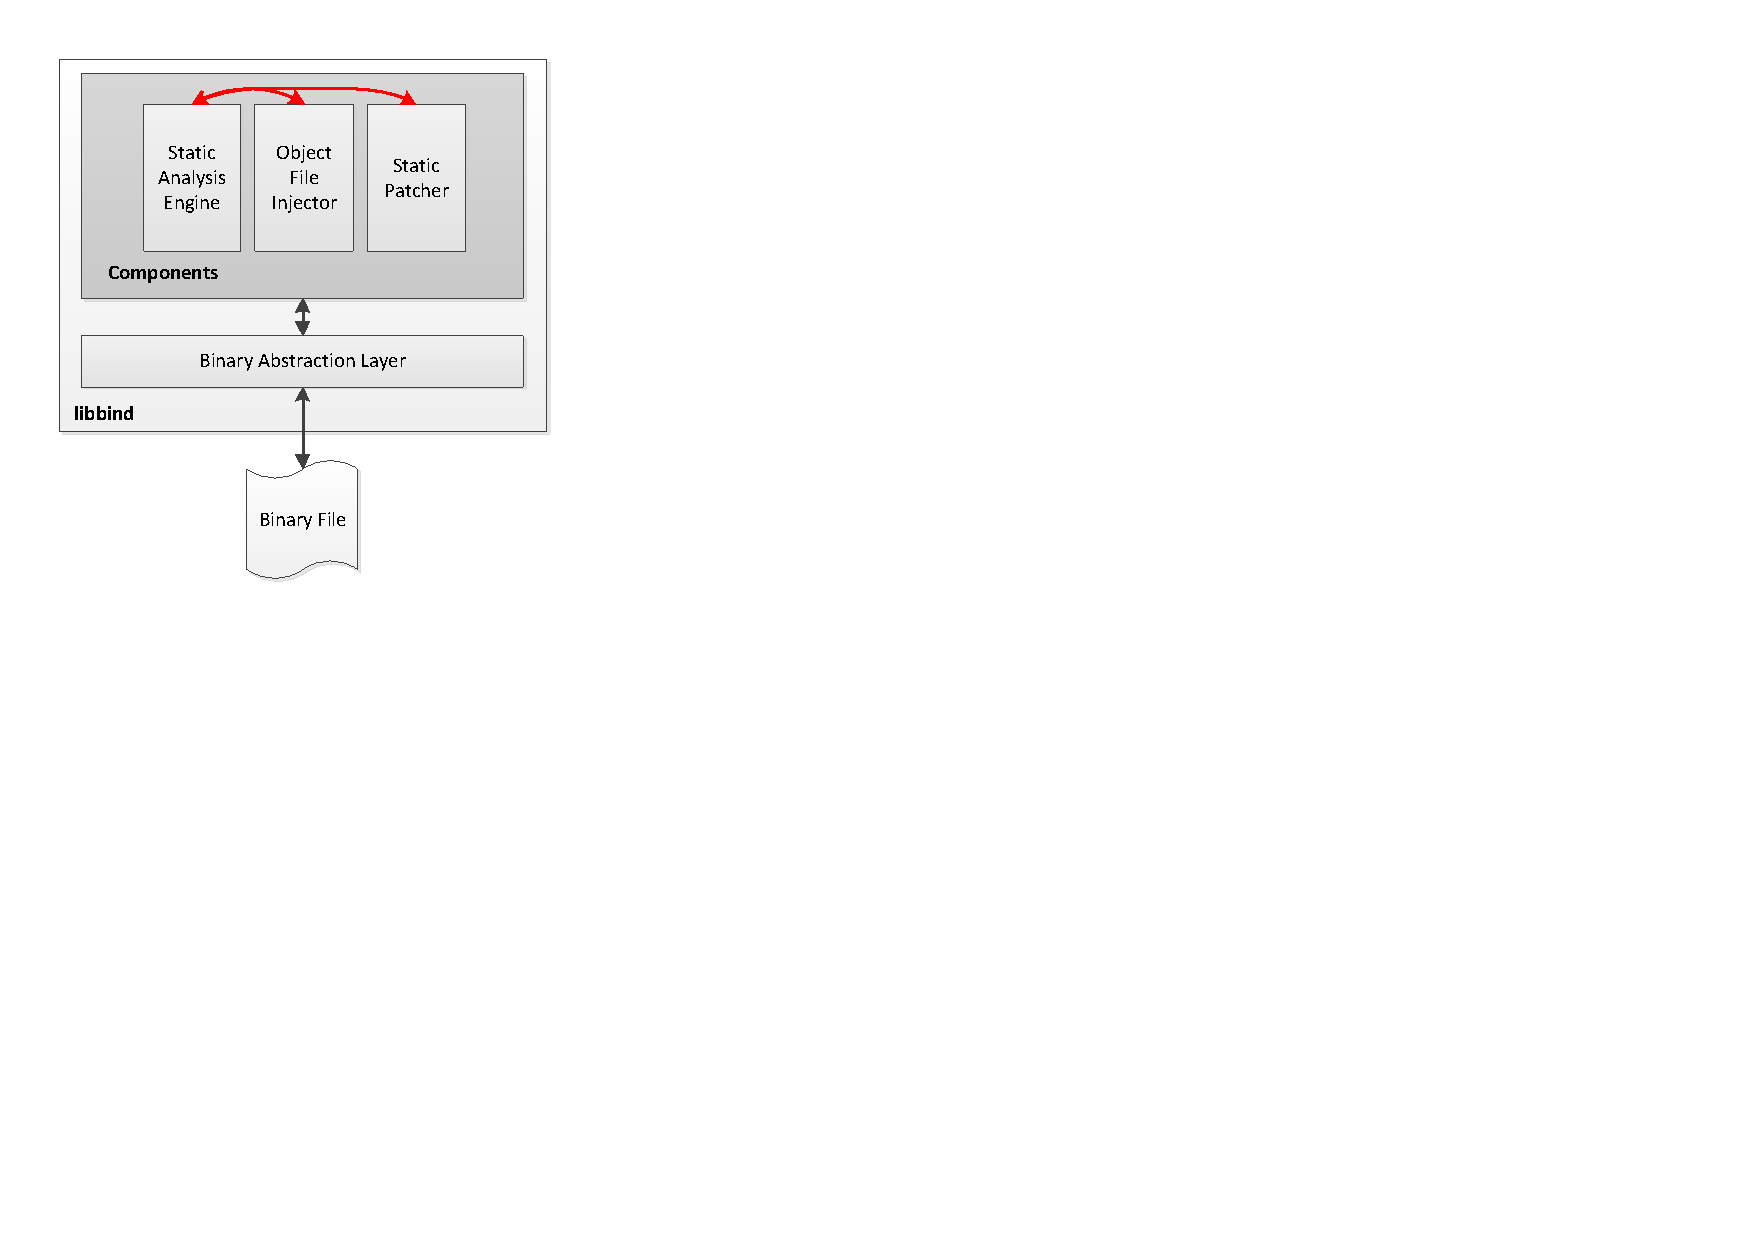
\includegraphics{Architecture.pdf}
 \caption[Architecture]{The high level architecture of libbind. The three components of libbind interact with a binary file through an internal binary abstraction layer. Within the library, the static analysis engine collaborates with the object file injector and static patcher.}
\end{figure}

The choice for the different components of libbind is mainly due to the natural and inherent separation in duty between the three aspects. The components interact through a well-defined interface which means the implementations are fully decoupled. This allows different implementations to be 'plugged in' increasing the portability value of the library. For example, it is trivial to write a static analysis engine plugin for a different architecture as long as the new implementation adheres to the original interface.

For now, we can treat the binary abstraction layer as libbind's internal representation of a binary file. Most importantly, the binary abstraction layer encapsulates the internal representation of the code of a binary as a CFG as required by \emph{(F4)} and \emph{(F5)} of the specification. As such, any modifications to the code of a binary are done through the addition, deletion or modification of nodes/edges in the CFG. Hence, a simplified and abstract way of considering each component of libbind is in terms of the operations it performs upon the CFG.

\section{Static Analysis Engine}

\begin{figure}[H]
 \centering
 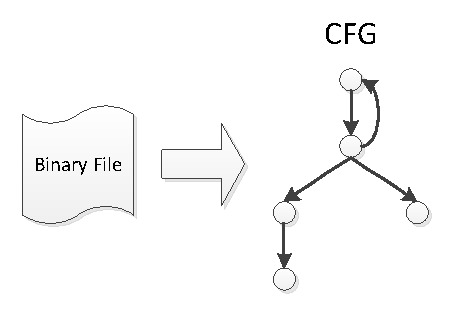
\includegraphics{Static_Analysis_Engine.pdf}
 \caption[Static Analysis Engine]{The primary role of the static analysis engine is to \emph{generate a CFG}.}
\end{figure}

While the fundamental goal of libbind is to provide static detouring, the usefulness of such a feature is greatly diminished without the appropriate supporting functionality. If a user were required to provide raw addresses to patch, it would not be feasible to use the library standalone. The static analysis engine essentially plays a supporting role which can be split into three parts:

\begin{description}
\item[Disassembler Engine] This is required for the construction of the CFG. The sole purpose of the disassembler engine is to perform the heavy lifting in terms of mapping the raw bytes of a binary to useful semantic information. For example, given an arbitrary address, the disassembler engine can disassemble the instruction held at that address and determine whether that instruction is a branching one and if so, decode the operand and attempt to figure out the branch destination.
\item[CFG Analysis] The generation of a CFG starts by pointing the disassembler engine to a root of disassembly (such as the entry point). Using the information provided by the disassembler engine, the analysis uses an algorithm to perform a depth-first discovery of the program structure.
\item[Symbol Table Parser] A symbol table is not guaranteed to exist in a binary because it can be completely stripped during or after compilation. The symbol table parser checks for the existence of a symbol table and if found stores the symbol information alongside the CFG.
\end{description}

To summarise, there are two phases to the static analysis performed by libbind. Firstly, a CFG is generated and then in the second pass, symbol information is added to the CFG. The CFG exposes an access interface through which a user is able to locate and express the source and destination for static patching. This is a concrete example of how the presence of a symbol table is beneficial. If we first consider a CFG without symbol information, the only way of identifying a basic block or function is to specify a heuristic in terms of instructions and iterate all basic blocks till a match is found. For example:

\noindent\begin{minipage}{\textwidth}
\begin{lstlisting}[language=C,caption={Identifying basic blocks via instruction heuristics}]
/*
 * Checks whether the first instruction is "push %rbp"
 */
struct bf_basic_blk * bb;

bf_for_each_basic_blk(bb, bf) {
  if(bb->insn_vec[0]->mnemonic == push_insn &&
      bb->insn_vec[0]->operand1->tag == OP_REG &&
      bb->insn_vec[0]->operand1->operand_info->reg == rbp_reg &&
      ...) {
    bf_trampoline_basic_blk(bf, bb, dest_bb);
    break;
  }
}
\end{lstlisting}
\end{minipage}

Basic block (and function) identification through instruction heuristics is verbose but necessary in order to be able to search at an instruction granularity. If available, a symbol table is a valuable resource that allows a far more convenient method of locating the same basic blocks/functions. Assuming the basic block we are searching for is actually the first basic block of a function named \emph{func1}, the identification could be expressed alternatively:

\begin{lstlisting}[language=C,caption={Identifying basic blocks via symbols}]
/*
 * Locates a function by its name.
 */
struct bf_func * func = symbol_find(&bf->sym_table, "func1");
bf_trampoline_func(bf, func, dest_func);
\end{lstlisting}

The functionality provided by the static analysis engine is powerful and can be used in many other applications. For example, it is possible to compare the CFG of two binaries to generate statistics for the number of changed functions/basic blocks/instructions. This is not a feature that is provided directly by libbind because it aims to be a general purpose library. It is a specific application of the static analysis engine and we demonstrate this as part of our evaluation.

\section{Object File Injector}

\begin{figure}[H]
 \centering
 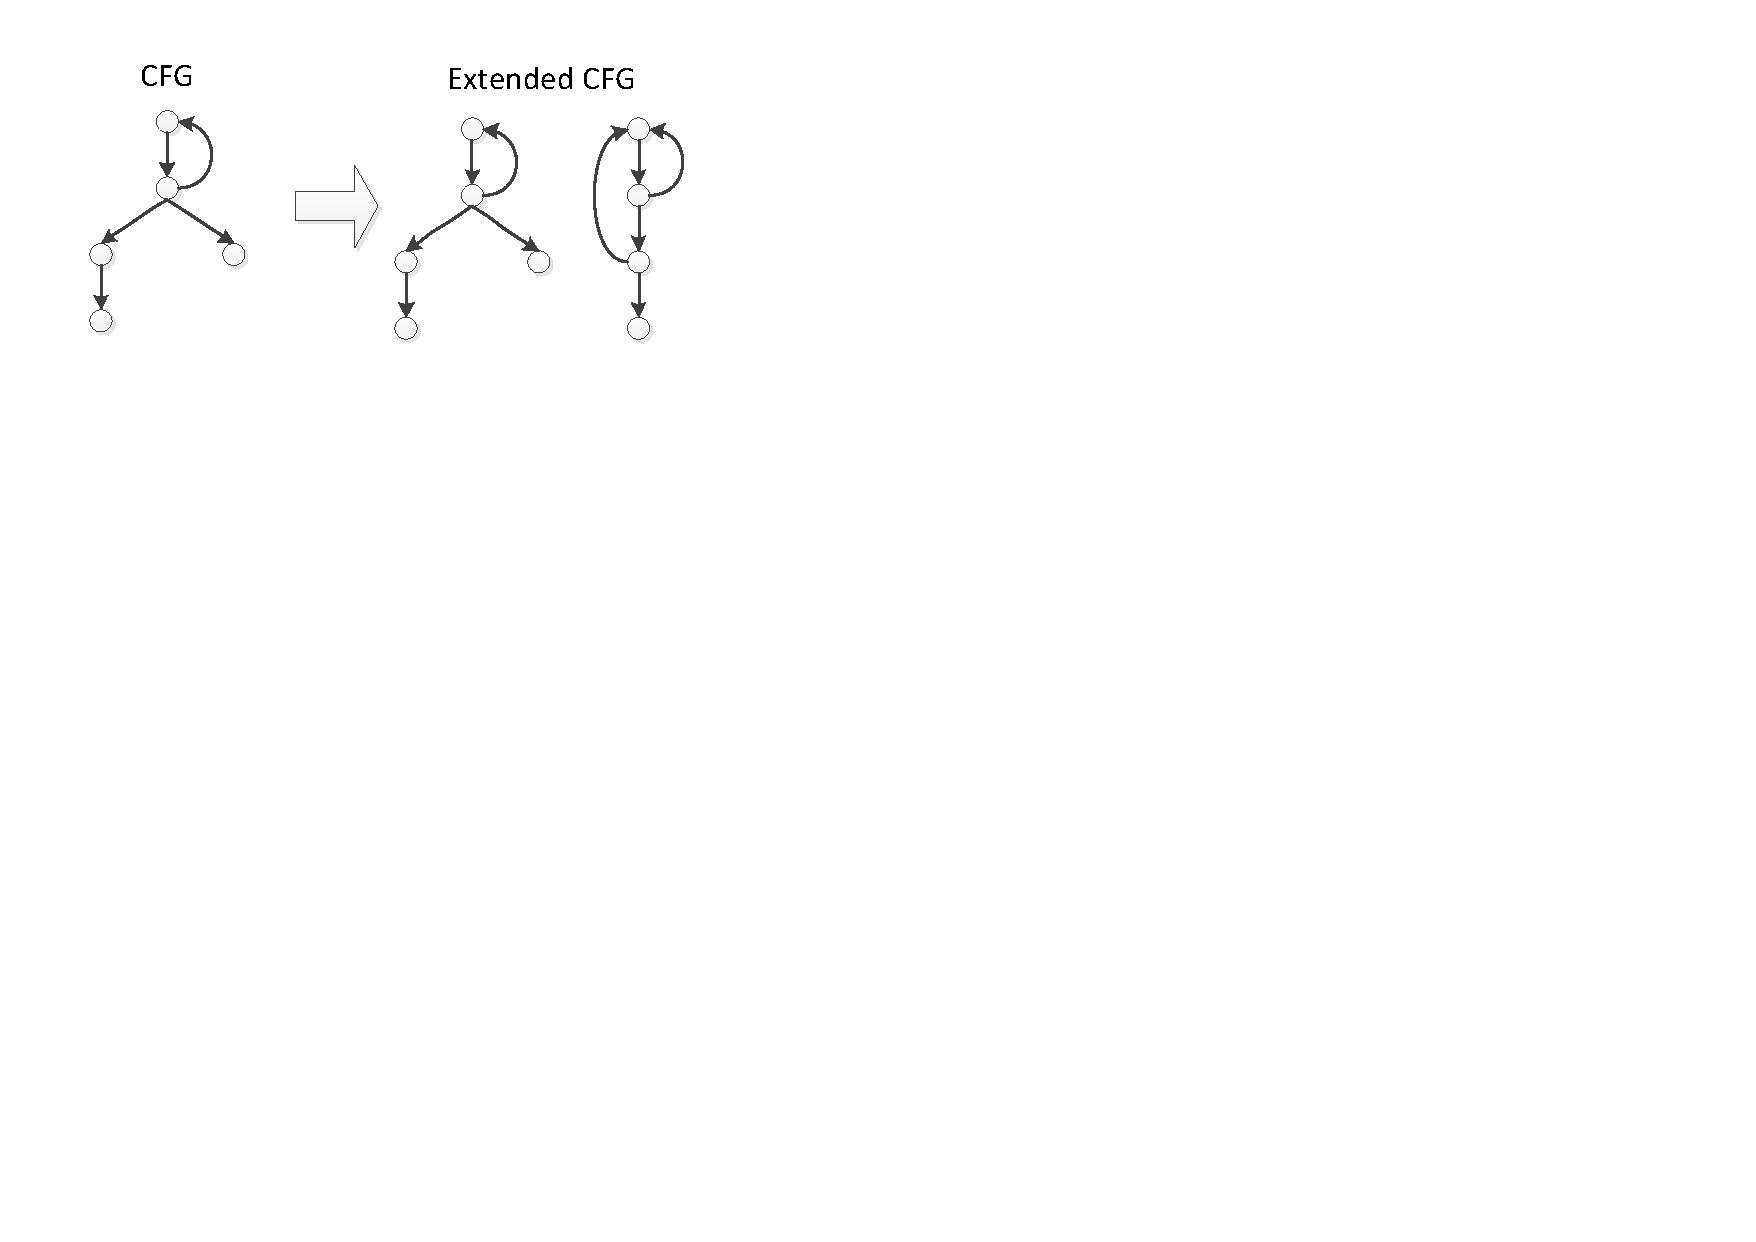
\includegraphics{Object_File_Injector.pdf}
 \caption[Object File Injector]{The role of the object file injector is to extend the CFG such that the CFG after injection is a superset of the CFG before injection. That is, a set of \emph{nodes and edges are added} which are disjoint to the original CFG.}
\end{figure}

The function of the object file injector is to load extra code into the target binary. Immediately after injection, the new code is unreachable from the original code which explains the two disjoint parts of the resulting CFG. The implication is that the injected CFG can be hooked up with the original CFG via the static patcher. Trampolining from the original code to the new code and back allows the semantics of target to be extended while preserving existing functionality.

The ability to load external code into the target binary is necessary in order to instrument the code at all. However, object file injection is a highly non-trivial process as we will see in later sections.

\section{Static Patcher}

\begin{figure}[H]
 \centering
 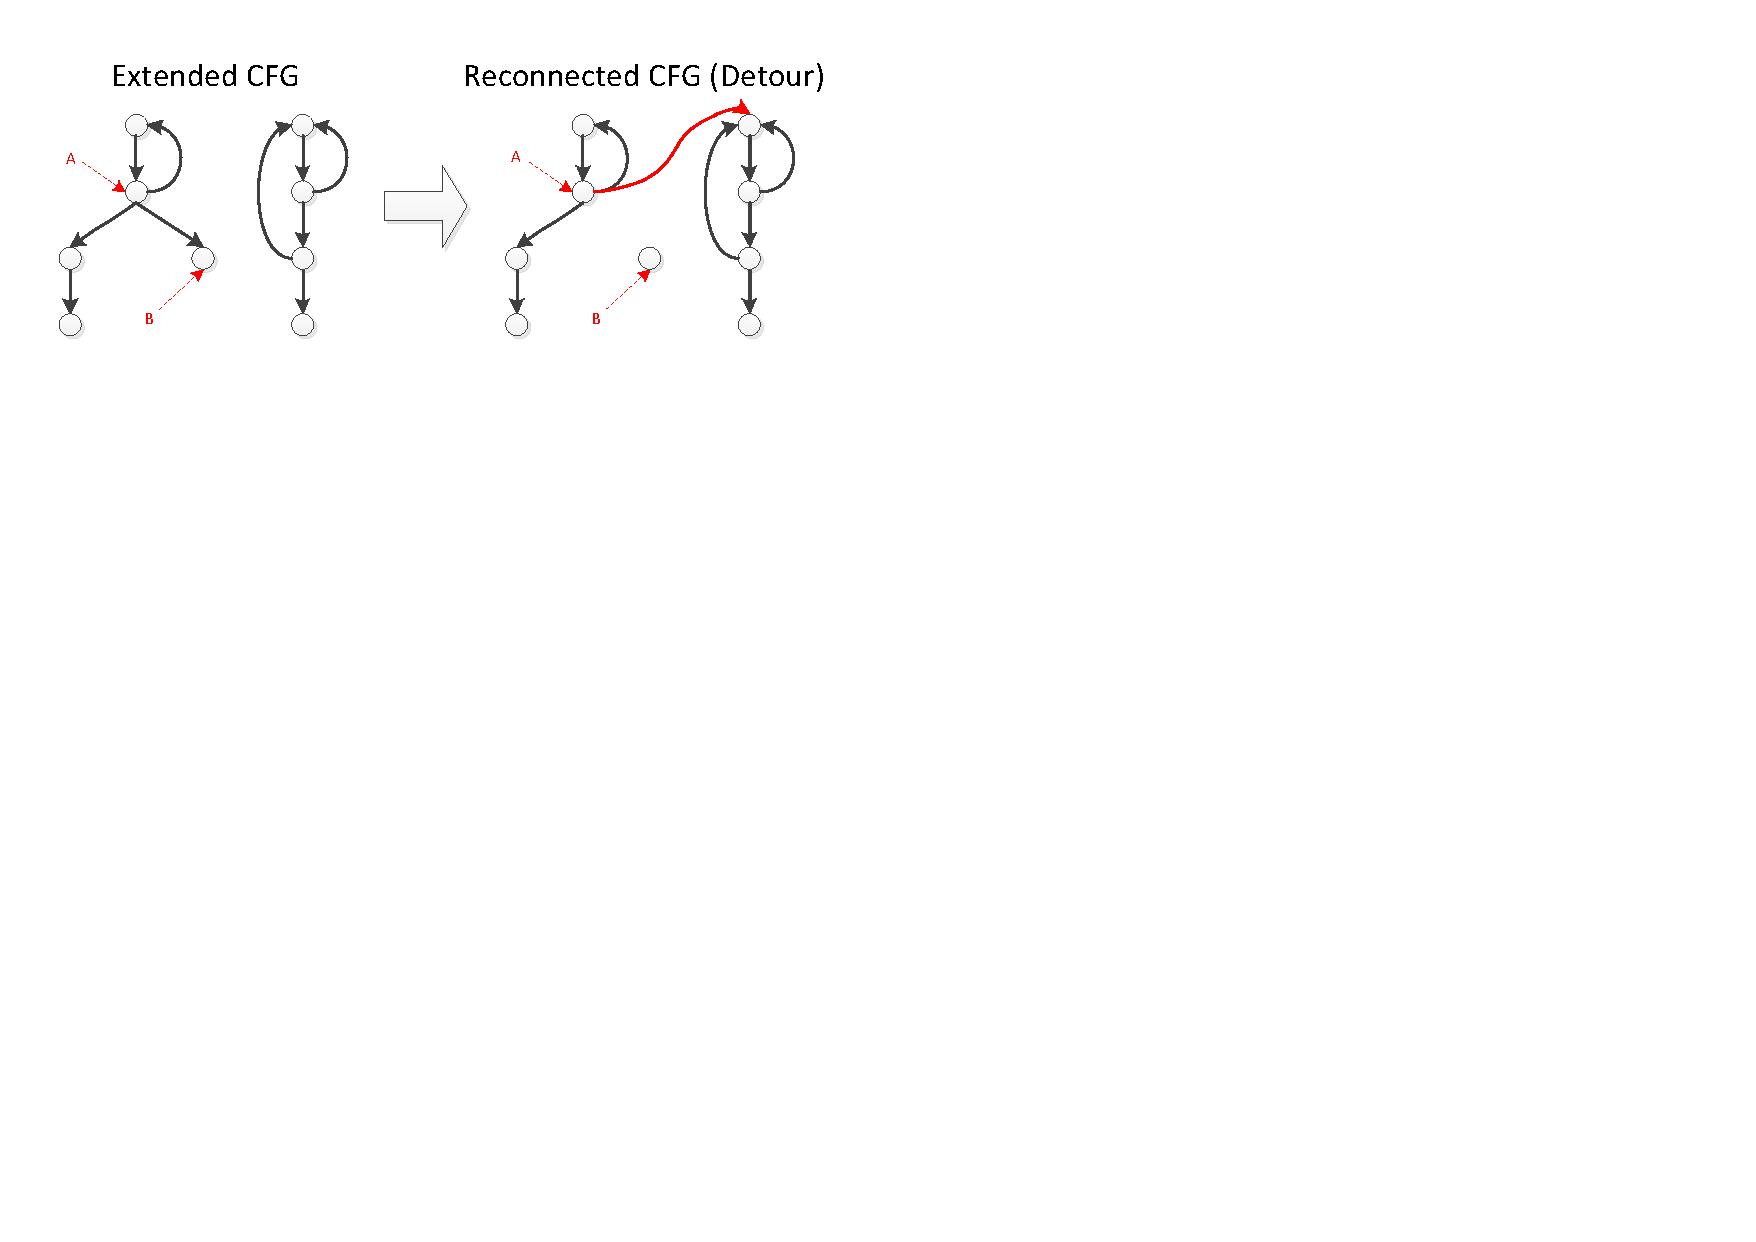
\includegraphics{Static_Patcher_Detour.pdf}
 \caption[Static Patcher Detour]{The role of the static patcher is to take a binary which is assumed to have all necessary code and manipulate its CFG to detour or trampoline execution. This is done by \emph{adding edges} to a CFG. This is the most basic case in which a single edge has been added to detour the execution of one basic block (\emph{A}) to another (\emph{B}). Note that the basic block \emph{B} is no longer reachable.}
\end{figure}

Similarly, the static patcher places a trampoline by adding two edges to a CFG - one to detour execution to the destination and another to trampoline back:

\begin{figure}[H]
 \centering
 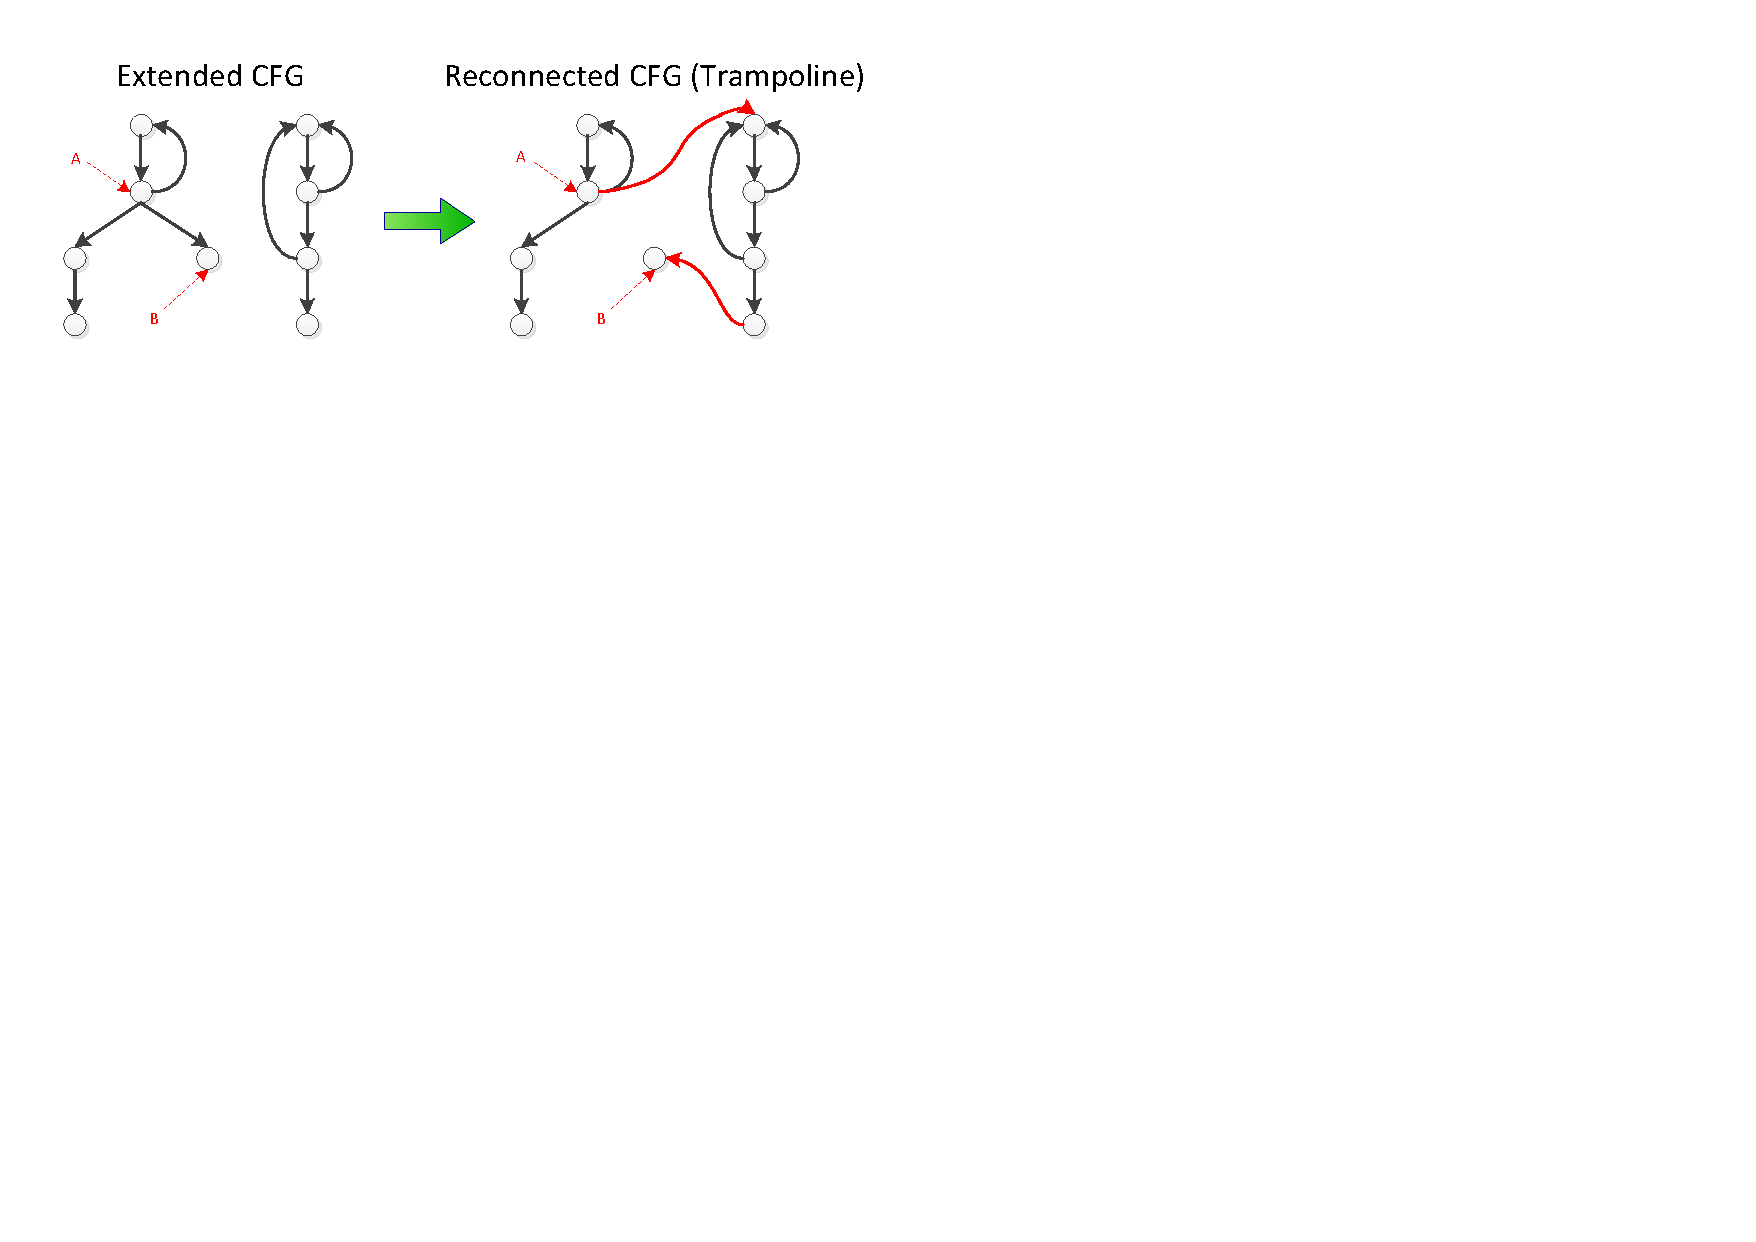
\includegraphics{Static_Patcher_Trampoline.pdf}
 \caption[Static Patcher Trampoline]{The static patcher adds two edges to the CFG to make a trampoline.}
\end{figure}

Strictly speaking, in our implementation, adding an outgoing edge to a CFG requires modifying the node the edge is to be added to. The intuition for this is that an edge simply represents a branch in the code so adding an edge writes a branch instruction to the start of a basic block. This is more of an implementation detail and in fact, we have already seen less aggressive methods of detouring execution which do not modify code in Chapter~\ref{chap:Background} (e.g. exception handlers).
\chapter{Implementation}\label{chap:Implementation}

In this section, we will discuss the implementation of each of the components of libbind. The workflow/usage is covered separately in Chapter~\ref{chap:Workflow}. Any major deviations from what has been covered in Design and Architecture will be highlighted.

\section{Binary Abstraction Layer}

The binary abstraction layer was originally designed to act as a bridge between the components and the target file. Essentially, libbind encapsulates a binary file in an internal structure called a \emph{bin\_file}. A \emph{bin\_file} contains two important elements: the BFD abstraction of a binary and its corresponding CFG (which is generated by the static analysis engine). In general, when a component needs to read information about the binary, it will read from the generated CFG. As we have seen, writing to the binary is equivalent to modifying the CFG. After a change to the CFG occurs, this change is flushed to the underlying binary through the BFD object. This was the original concept but it had to be modified to work in practice. Figure~\ref{fig:BAL_Attempt1} illustrates the original approach to creating the binary abstraction layer.

\begin{figure}[H]
 \centering
 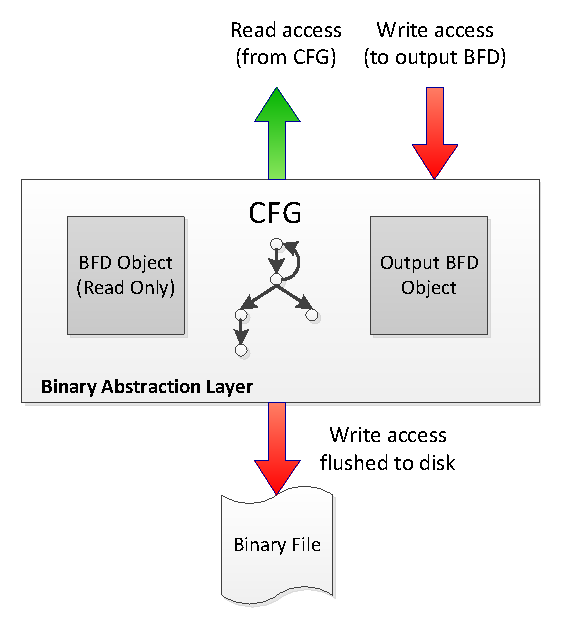
\includegraphics[scale=0.86]{Binary_Abstraction_Layer_Attempt1.pdf}
 \caption{The original approach for the binary abstraction layer. The read only BFD object is the abstraction of the original binary file. The CFG is generated from this BFD. Any changes need to be outputted to the output BFD independently.}
\label{fig:BAL_Attempt1}
\end{figure}

\subsection{Original Approach}

The problem with the original design was that it only encapsulated a single BFD object. With libbfd, it is possible to open a file in two ways:

\begin{enumerate}
\item An existing file can be opened with read-only access.
\item A \emph{new and empty} file can be opened with write access.
\end{enumerate}

This restriction of libbfd is by design, but does not make it ideal for patching. Tools such as \emph{ld} and \emph{objcopy} work well above libbfd because the files they output are written in a single pass. Although BFD is unsuitable for our usage, it is possible (albeit very awkward) to patch a binary file. Figure~\ref{fig:BAL_Approach1} illustrates the steps required to patch a file through libbfd:

\begin{figure}[H]
 \centering
 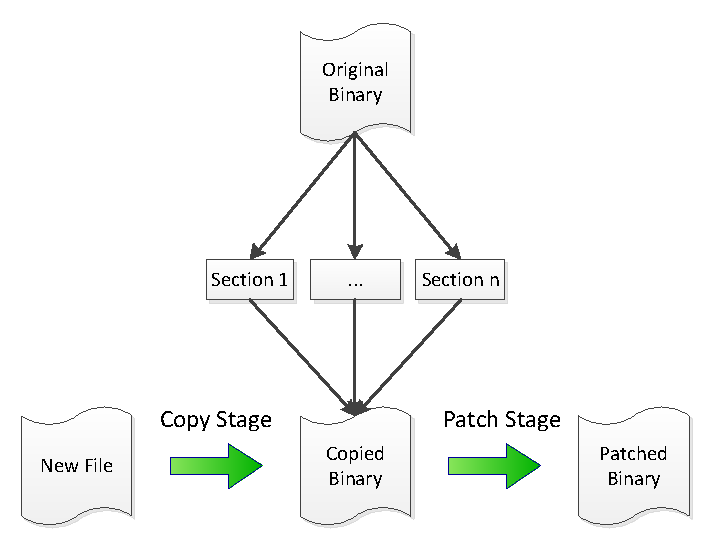
\includegraphics{Binary_Abstraction_Layer_Approach1.pdf}
 \caption{The process required to patch a file using libbfd.}
\label{fig:BAL_Approach1}
\end{figure}

The abstraction used within BFD is that an object file has:

\begin{itemize}
\item A header
\item A number of sections containing raw data (this data could represent code)
\item A set of relocations
\item Symbol information
\end{itemize}

As illustrated, patching a binary file with libbfd works through a series of steps:

\begin{enumerate}
\item The original binary must first be opened with read access.
\item A new BFD (which starts off empty) is created. The original binary is then reconstructed in this BFD by extracting the four different types of content (as defined above) and copying them. This reconstruction all happens in memory.
\item Before the new BFD object is flushed to disk, the user is able to perform patches by editing the contents of sections.
\item After all patches are performed, the BFD object is flushed to disk. If more modifications are needed after this, the entire process has to be restarted.
\end{enumerate}

In terms of the implementation of this algorithm, the first two stages are essentially what objcopy does. Our implementation of static patching re-uses the objcopy code for the decomposition and reconstruction stage. The rest of the algorithm is trivial to implement. However, there are two drawbacks with this method:

\begin{enumerate}
\item The part of the code re-used from objcopy is large, approximately 1.5 KLOC.
\item BFD is merely an abstraction over many file formats. This means that it represents a more generalised abstract format. Unfortunately, it does not encapsulate all the information required for the full reconstruction of a binary. In order to obtain this information, the code relies on a dependency with the file format and ends up calling functions in libelf.
\end{enumerate}

\subsection{Final Approach}

Given the disadvantages of using the method from the original approach, there is no reason to use BFD to perform the patching. The method is overly complicated and more error-prone simply because of the amount of code that has to be written to perform a patch. Since a dependency on libelf is unavoidable, we can re-implement the solution by using libelf directly and save the hassle of forcing libbfd to do something it was not designed for. In terms of the binary abstraction layer, this means that we modify write accesses to directly modify the disk version instead of through the BFD object as seen in Figure~\ref{fig:BAL_Final}:

\begin{figure}[H]
 \centering
 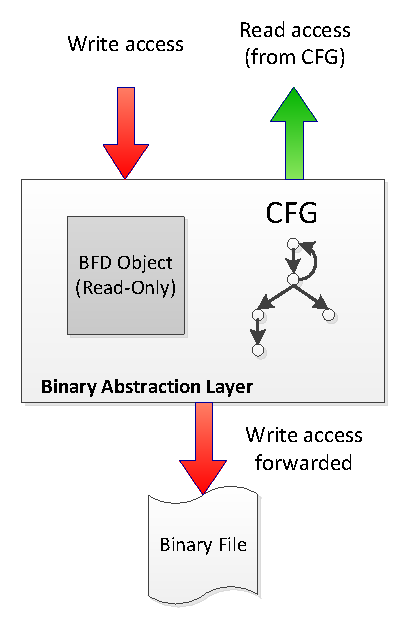
\includegraphics{Binary_Abstraction_Layer_Final.pdf}
 \caption{The final design for the binary abstraction layer. Read accesses are handled in the same way but in this design, we have removed the output BFD. Write accesses are alter the target binary file directly.}
\label{fig:BAL_Final}
\end{figure}
 
In the final implementation of the binary abstraction layer where libelf is used, the same result as with the original approach can be achieved in under 100 LOC. The method is fairly intuitive and the concept is visualised in Figure~\ref{fig:Loading_Binary}:
 
\begin{figure}[H]
 \centering
 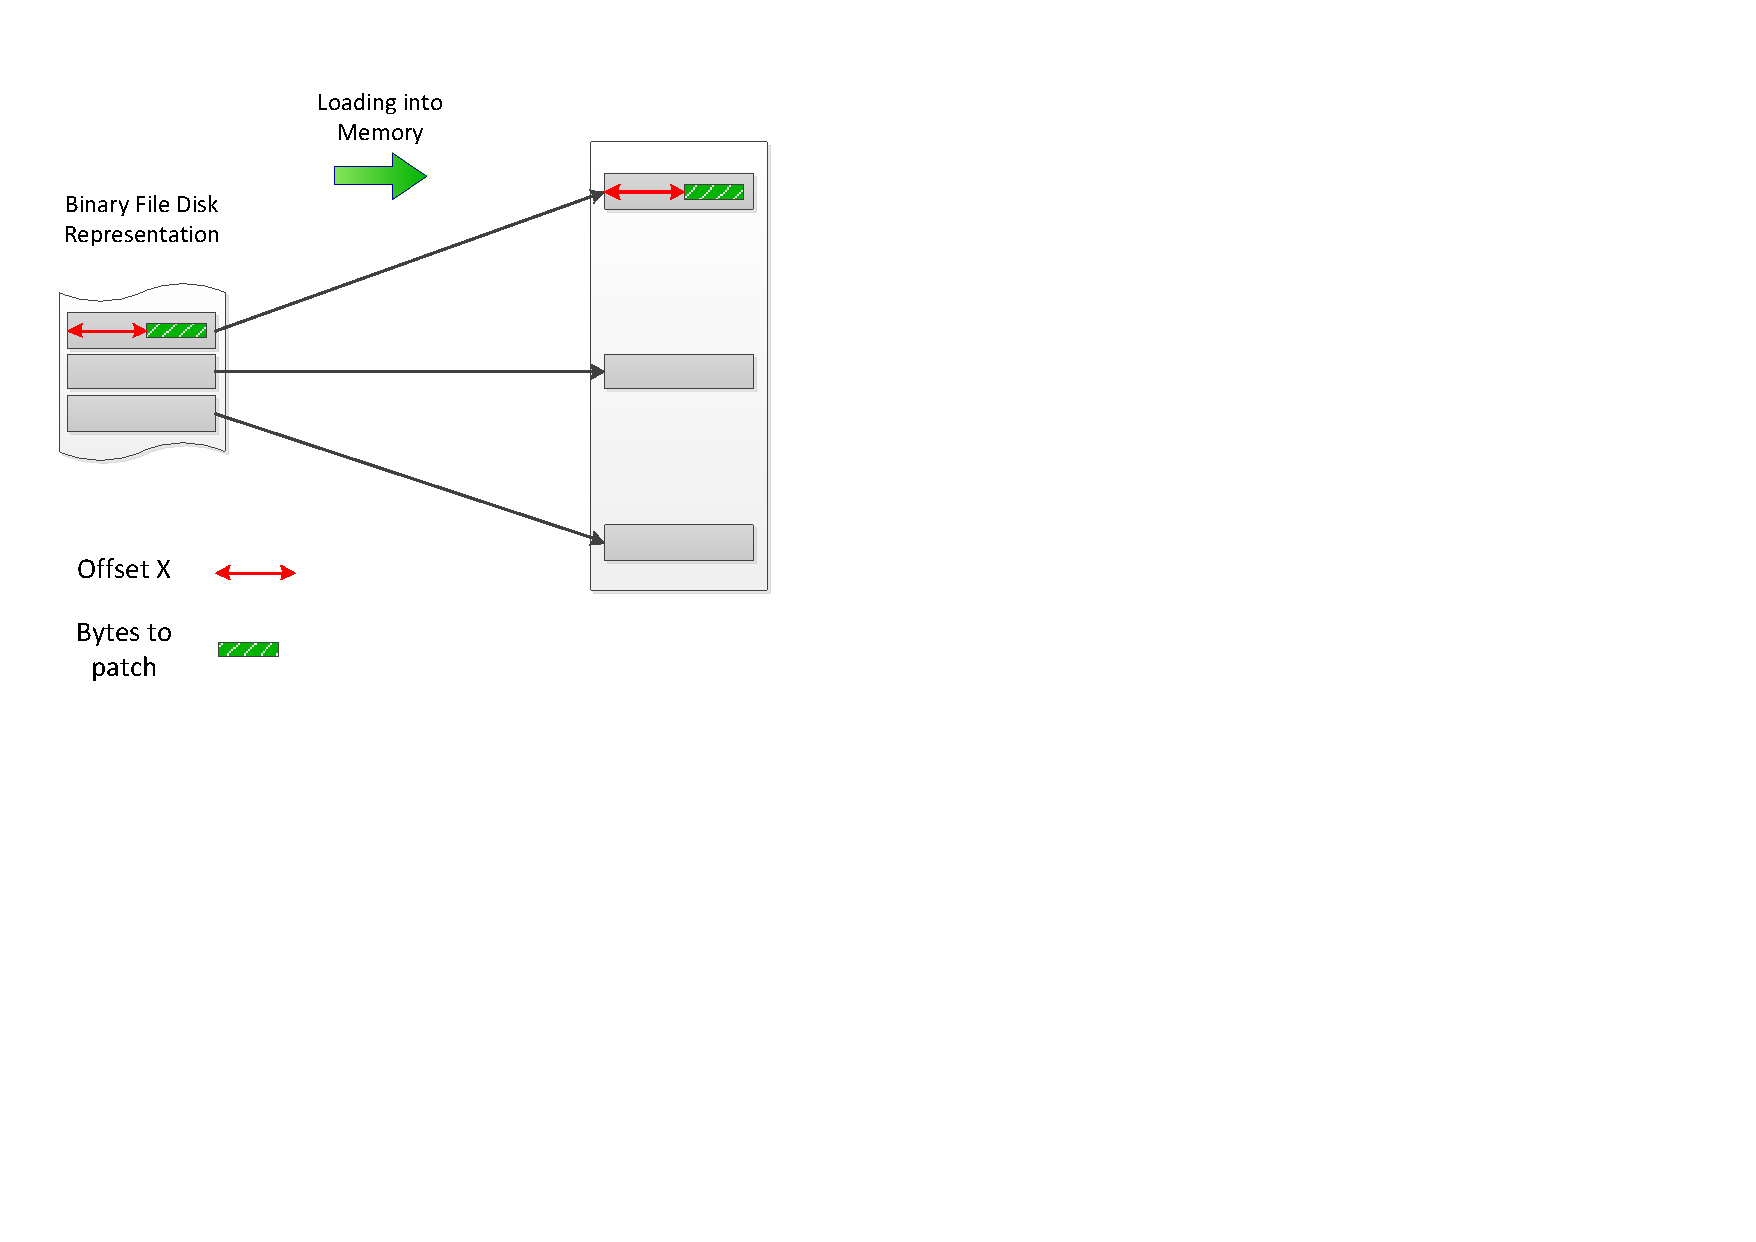
\includegraphics{Loading_Binary.pdf}
 \caption{The concept of how patching works in the final implementation. The most important idea here is that a section in the disk representation is preserved (not split) when it is mapped into memory. This means data that is at a certain offset into the section in the disk representation will be offset by the same amount after loaded into memory.}
\label{fig:Loading_Binary}
\end{figure}
\todo{add label for the loaded executable (memory)}
 
In libelf, similarly to libbfd, an executable contains a set of sections in which both code and data can reside. When the operating system loads the executable into memory, each section is based at some base address. We can reverse this to map a virtual memory address to a physical file offset. If a physical file offset can be found, the bytes can be patched as a regular file.

\begin{enumerate}
\item First, the section header of the executable is parsed with libelf. This allows us to obtain a set of sections and most importantly, for each section libelf can tell us three things:
  \begin{description}
  \item [Section size] The size of the section.
  \item [Section base address] The address that the section will be based at when the executable on disk is loaded into memory.
  \item [Section disk offset] The disk offset of the section.
  \end{description}
\item By iterating through the section information extracted in the previous step, it is possible to find out what section an arbitrary virtual memory address is contained in. During patching, the memory address we are interested in is the address of the code at which a detour is to be written. The offset of the virtual memory address into the section can be calculated by:

\textbf{(virtual\_memory\_address - section\_base\_address)}.
\item Therefore, the disk offset of the virtual memory address can be calculated by:

\textbf{(section\_disk\_offset + (virtual\_memory\_address - section\_base\_address))}.
\end{enumerate}

This process allows an arbitrary virtual memory address to be mapped to its corresponding disk file offset. This offset can then be patched with regular C file IO functions such as \emph{fopen}/\emph{fseek}/\emph{fwrite}/\emph{fclose}.

Fortunately the architecture of libbind was designed such that a change in the implementation of one component (even if that is the binary abstraction layer) would not impact the other components. The downside is that a lot of time was lost writing the BFD patch code, only to have it thrown out in favour of another method. However, this was unavoidable as the documentation did not make it clear how difficult the implementation of patching would be. The lack of clear documentation is a widely recognised drawback to libbfd and the required steps were only discovered by reading through the objcopy source.

\section{Static Analysis Engine}

As discussed in earlier sections, the static analysis engine allows libbind to discover the code of a binary. It is implemented in several layers and matches the design described in Design (Chapter~\ref{chap:Design}). Figure~\ref{fig:SAE_Detail} shows the internal implementation of the static analysis engine in more detail:

\begin{figure}[H]
 \centering
 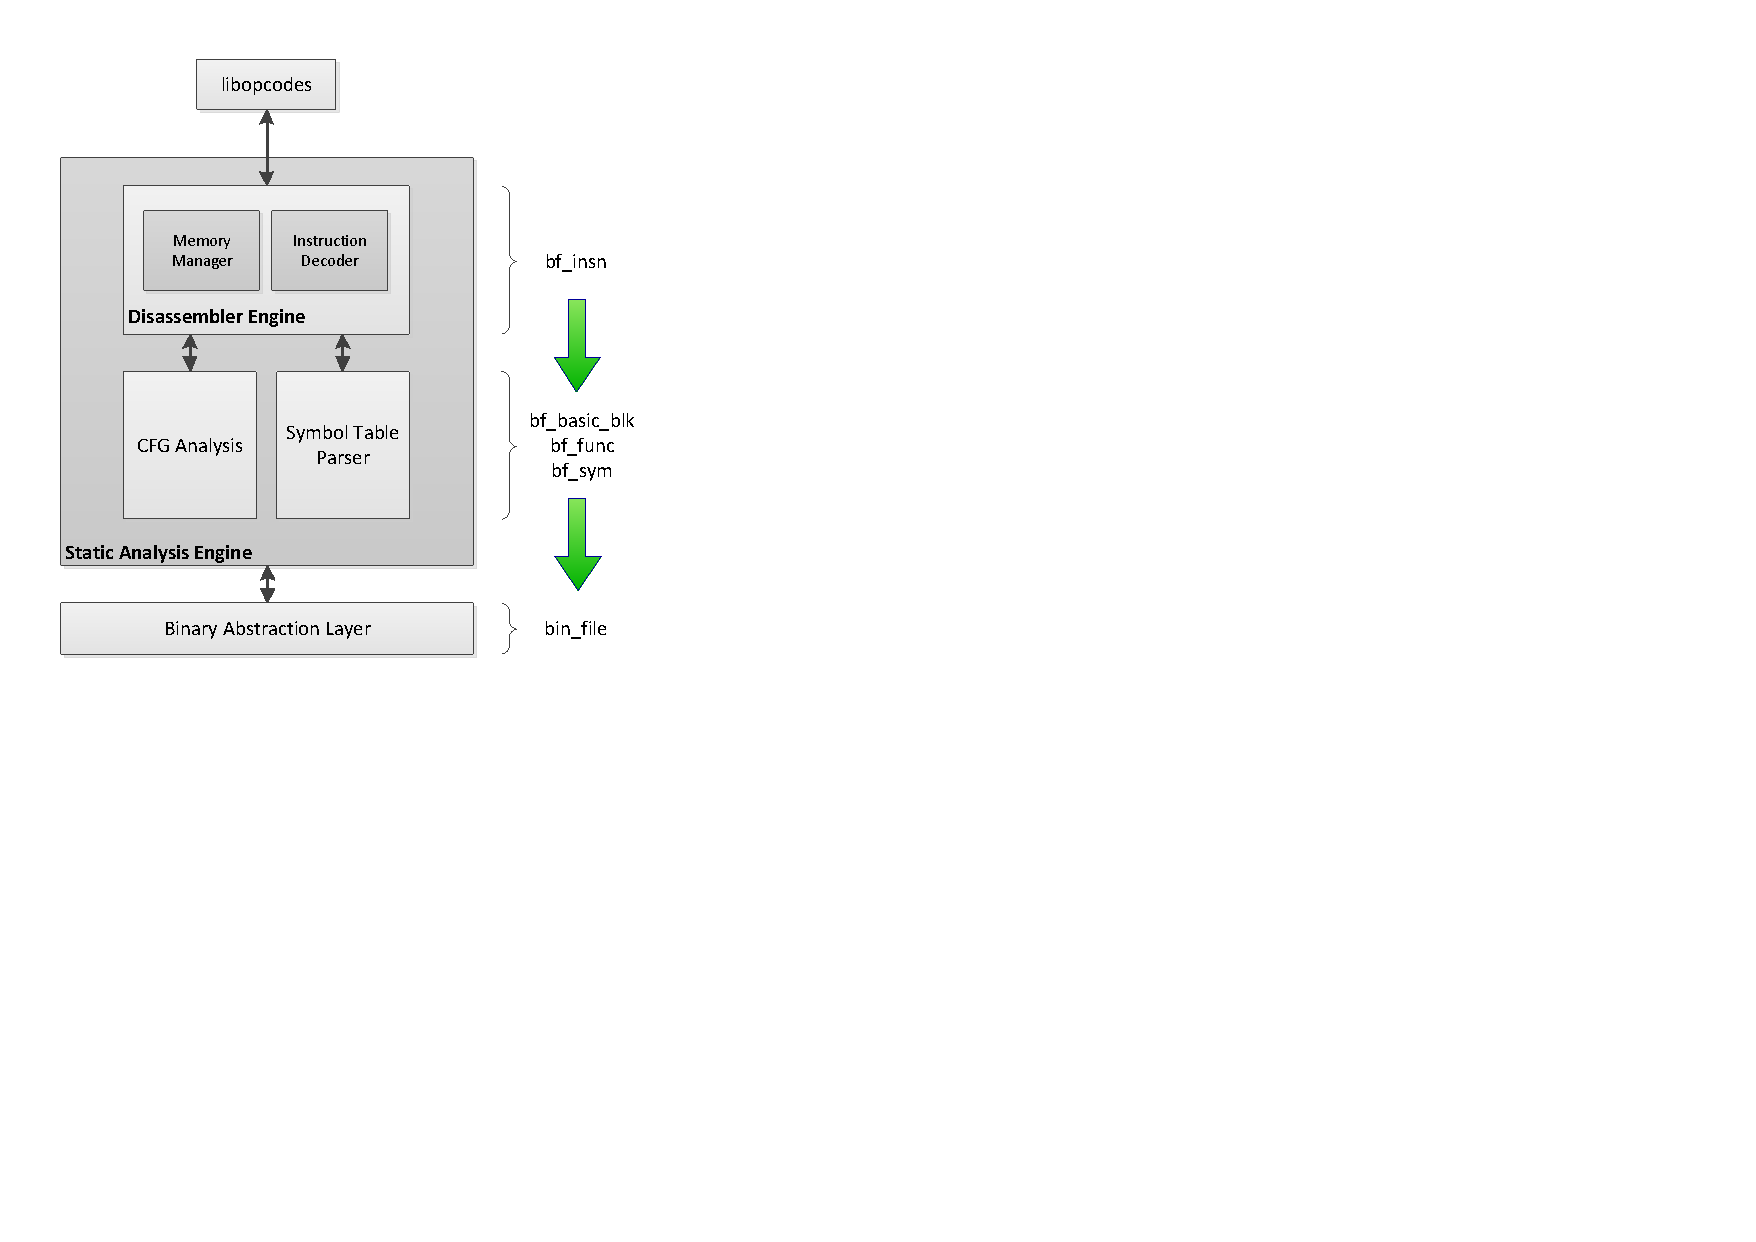
\includegraphics{Static_Analysis_Engine_Detail.pdf}
 \caption[Hierarchy]{The internal implementation of the static analysis engine.}
\label{fig:SAE_Detail}
\end{figure}

In order to understand how the static analysis engine works as a whole, we will explain each component in further detail.

\subsection{Disassembler Engine}

In practice, the disassembler engine is responsible for parsing and translating the strings received from libopcodes and storing the information in its internal semantic representation. At the most basic level, a \emph{bf\_insn} corresponds to an assembly instruction. In order to use libopcodes, we first needed to solve the two problems outlined in Design:

\begin{description}
\item [Limited disassembly scope] libopcodes can only disassemble a single address at a time which means the same applies for the disassembler engine. In order to make the disassembler engine useful, CFG analysis needs to be performed when an instruction is disassembled. The results of this analysis will then be used to drive the disassembler engine. For example, if the CFG analysis comes across a conditional branch instruction, it will need to instruct the disassembler engine to disassemble both the branch target and the next instruction. This analysis will be covered in detail later since it is not part of the disassembler engine.
\item [Output redirection] The default behaviour of libopcodes is to print to a stream using \emph{fprintf}. It is possible to override this behaviour by instructing libopcodes to invoke a custom function with the same prototype as fprintf.
\end{description}

One quirk of libopcodes is that it invokes the fprintf function (or overridden substitute) for each of the following `types': mnemonic, operand, separator and comment. As a concrete example, consider the following instruction:

\noindent\begin{minipage}{\textwidth}
\begin{lstlisting}[language={[x86masm]Assembler},caption={Example instruction disassembled by libopcodes.}]
ucomiss 0x9124(%rip), %xmm0 # 414d58
\end{lstlisting}
\end{minipage}

The custom fprintf function is invoked 4 times with the following:

\noindent\begin{minipage}{\textwidth}
\begin{lstlisting}[language={[x86masm]Assembler},caption={Strings received by custom fprintf. Type information is included for the benefit of the reader but is not given by libopcodes.}]
ucomiss (Mnemonic)
0x9124(%rip) (Operand)
, (Separator)
%xmm0 (Operand)
# (Separator)
414d58 (Comment)
\end{lstlisting}
\end{minipage}

One option is to concatenate all these instruction parts to obtain a full instruction but we already decided in Design that we would not store instructions in string form. Instead, the implementation stores semantic information about each instruction as it is disassembled by libopcodes. An issue with this is that libbind needs to know how to decode every type of string it receives. For example, an arbitrary string that is received might be a mnemonic, operand, separator or comment. It would be very inefficient to attempt to decode each string to determine what type it should be. libbind solves this issue by implementing a finite state machine which allows it to know what type it is expecting to receive:

\begin{figure}[H]
 \centering
 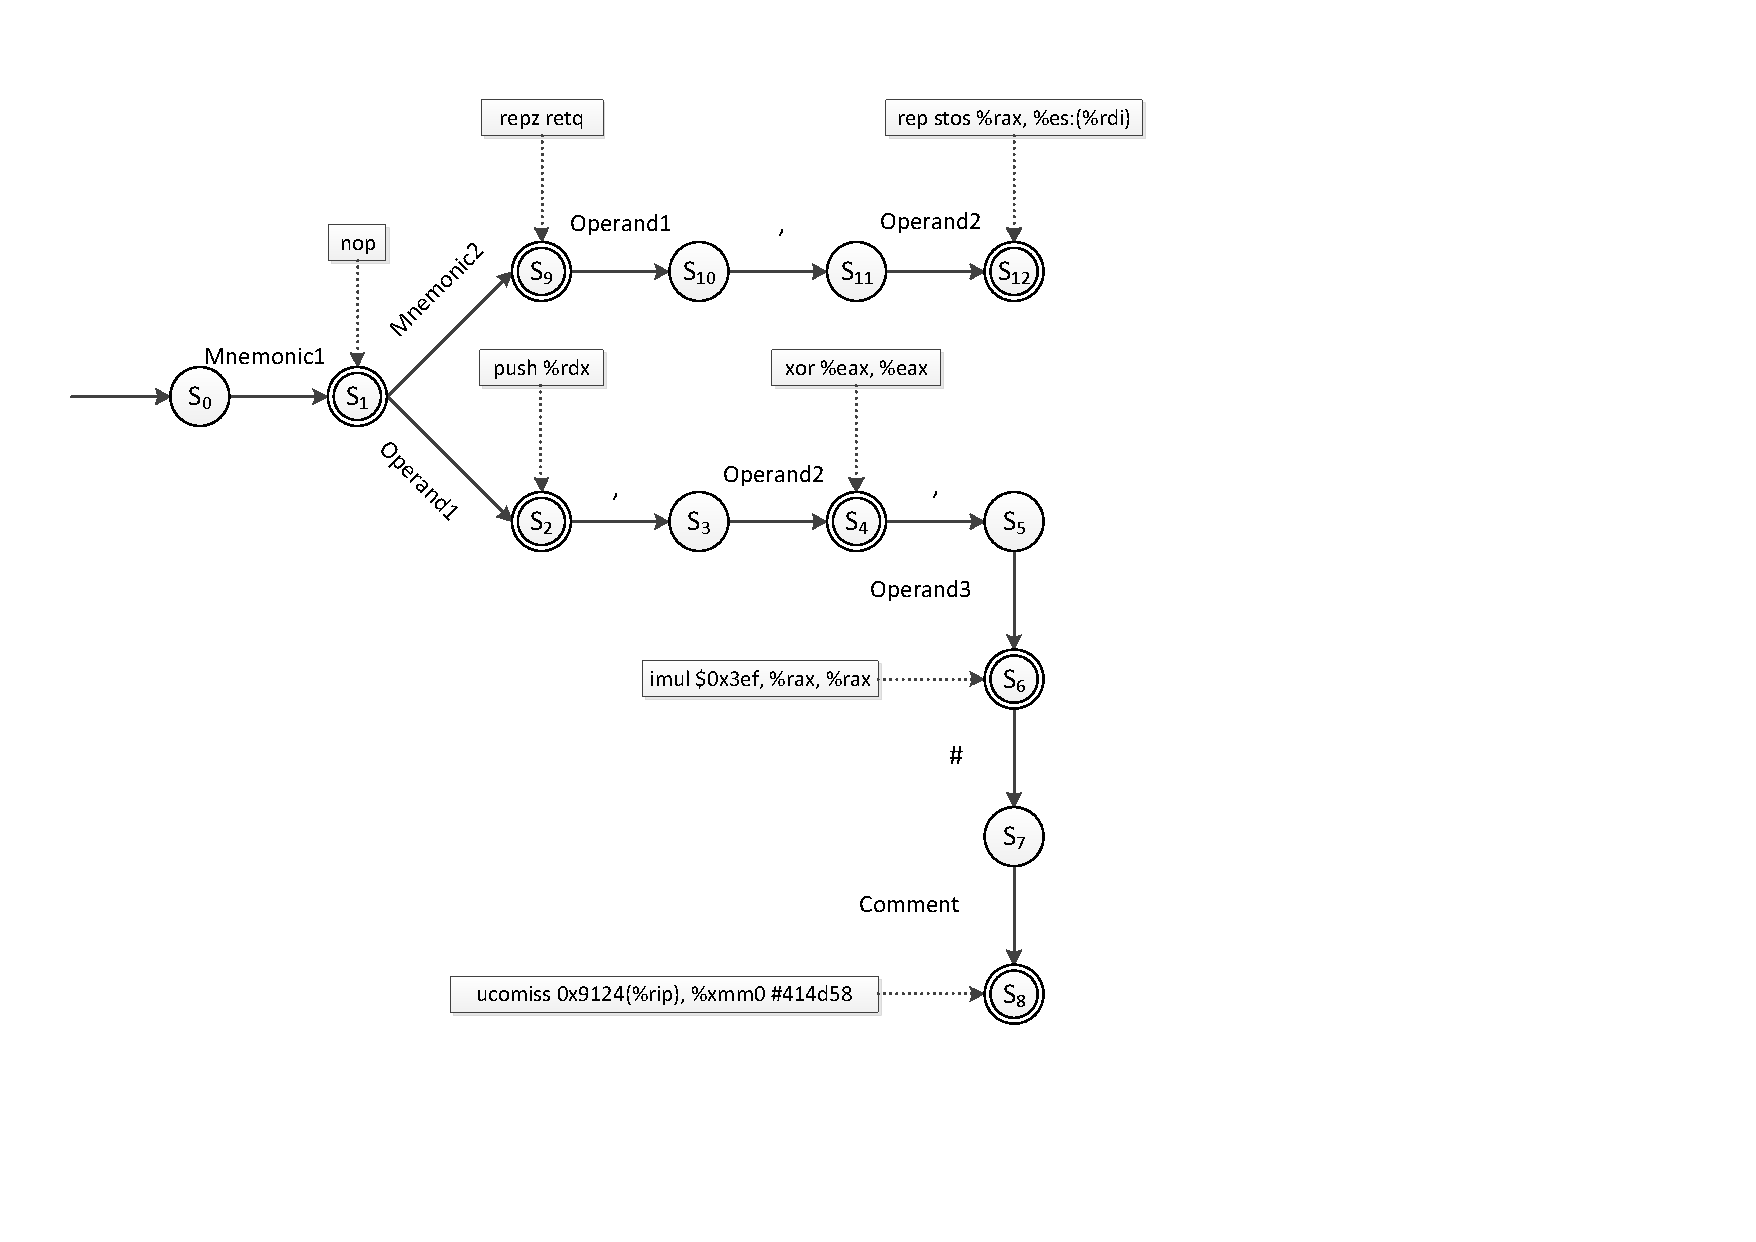
\includegraphics[scale=0.8]{Instruction_State_Machine.pdf}
 \caption[Hierarchy]{The instruction finite state machine used by the disassembler engine to determine how the received string should be decoded. A double circle denotes a possible terminal state. For each terminal state, an instruction which would cause termination at that state is shown.}
\label{fig:Instruction_State_Machine}
\end{figure}

\todo{This diagram might have to be redrawn to take up less horizontal space so it can be sized larger.}

Each time a new instruction is disassembled, a new bf\_insn object is constructed and the current state is restarted to the initial state of the instruction finite state machine. When fprintf is called, the received string is decoded based on its expected type, the semantic information updated for the bf\_insn and the current state of the state machine advanced. $S_1$ is a special case because two types can be received at this point: an operand or a mnemonic. In this case, we can only decode as one type and if that fails decode as the other type. Since an operand is more common, the disassembler engine attempts to decode as that first. The implementation of the instruction decoder is covered later.

\subsubsection{Memory Manager}

\subsubsection{Instruction Decoder}

\subsection{CFG Analysis}

\subsection{Symbol Table Parser}


%in practice, the disassembler engine is responsible for parsing and translating the strings received from libopcodes and storing that information in its internal semantic representation (bf\_insn, bf\_basic\_blk). bf\_func can be identified from three ways only:
%1) if it is the target of a call site
%2) if it corresponds to an address identified as a bf\_sym
%3) if the user defined it as a root for cfg generation and explicitly stated it is a function (cfg analysis and generation is covered in depth in...)
%
%further information such as size of symbols (which tells us size of function) is available because we are parsing the symbol table directly from libelf.
%
%quirks of libopcodes disassembler such as how it passes us the instruction parts (mnemonic, operands, separator) as strings! we build a finite state machine which allows us to 
%
%we can draw finite state machine in diagram here
%
%binary\_file
%
%within a binary\_file, there are 2 levels of code representation. firstly we have bf\_basic\_blk which represents a basic\_block as defined in architecture.
%
%binary\_file is composed of a CFG of bf\_basic\_blk objects. during the process of cfg generation and after it completes, we add extra information. i.e., bf\_func 'labels'
%
%bf\_func
%
%implementation of CFG analysis and generation...
%
%epilogue relocation

\section{Object File Injector}
\section{Static Patcher}

%
%distribution and documentation
%
%automake which we use to deal with library dependencies (libelf, libbfd, libopcodes, libkern).
%
% and doxygen
%
%WORKFLOW

%\chapter{Project Plan}

%If time permits, the most desirable extension is to add dynamic detouring to the library. %We would implement some form of runtime detouring and provide users with the option to %choose between both methods. Another smaller extension which would also be useful is to %allow the library to be invocable through the command-line as well as through the API (as %seen with ELFsh).
\chapter{Deviations from Design}\label{chap:Deviations}
\chapter{Workflow}
\chapter{Testing}

%TESTING
%
%we want to test robustness and reliability of the library. several areas in particular:
%
%- we want make sure the library is scalable and does not fail on large scale systems. we test on real-world systems, as opposed to toy examples. namely, we test against coreutils (includes stuff like ls, cp, rm, etc.).
%
%we have a suite of regression tests which test the following:
%
%test 1: coreutils\_test32/64
%
%so firstly we want to test the successful disassembly and cfg generation for some real-world example. 
%
%probably want to use valgrind to check for errors
\section{Evaluation}

One of the easiest ways to evaluate the success of the project is prove that we are able to trace function calls as we discussed in the Introduction. Given a target program, we want to be able to print out all occurrences of invocations of its functions. A specific example we want to test against is another lighttpd bug\footnote{Bug \#2169 (http://redmine.lighttpd.net/issues/2169)}. Although this bug is currently resolved, the original issue took around 8 months to locate and fix. Our library should allow us to instrument an old version of lighttpd to provide logging of:

\begin{enumerate}
 \item \textbf{Procedure invocations} - We should be able to gather information about the function calls leading up to the bug occurring. This will require \emph{(F1)} and \emph{(F2)}.
 \item \textbf{Procedure return values} - If we are able to find the call convention used for the application, we will be able to instrument code at the return address of functions to read off a particular register's value which should be holding the return value. This will require \emph{(F3)}.
 \item \textbf{Procedure arguments} - If we instrument code at the start of a function, we should be able to inspect the stack and log the values of the arguments.
\end{enumerate}

\emph{(F4)}, \emph{(F6)} and \emph{(F7)} are implicit requirements, but it is possible for us to evaluate \emph{(F5)} by targeting the library against two versions of lighttpd (before and after fix), and accessing the generated CFG to print out the code differences.

Since our approach is similar to EEL's, we can also measure our success by quantitatively comparing the overhead added by the library. As we saw earlier, EEL creates a markup from 8KB to 350KB. We believe we can make an improvement on this and we can easily compare results as a way of evaluating our library.
\chapter{Conclusion}\label{chap:Conclusion}

\bibliographystyle{plain}
\bibliography{refs}

\end{document}
